\section{Case Studies}
In this section, we explain with the help of case studies the effectiveness of our clustering method to identify relevant samples and discuss few malicious cases that we encountered during our analysis and the relation between them.

\subsection{Phishing Via WPN Ads}
This case study discusses how Web Push Notification(WPN) service is being used by some adversaries to deliver spoofed pages to the end users. In traditional phishing method, the success rate of an adversary in delivering phish links to the users is quite low as they have to overcome multiple defenses to reach the end user. However, advertisements that are sent using WPN are delivered directly to the user without any additional filtering/monitoring done by Ad blockers. Few cases that we encountered from one of the result clusters contained advertisements that led to spoofed pages of popular news websites such as CNN, Fox News and Entertainment Today. This phenomenon could be observed from Fig.\ref{fake_news}. To be specific, the domains of these landing pages are \texttt{appearsnews.com(bottonm-left),  producednews.com(top-left), usa-health-news.com(center \& bottom-right)} and \texttt{ healthydreamstoday.com(top-right)}. It has to be noted that the domain \texttt{usa-health-news.com} serves spoofed pages of two different news sites. Further analysis of these cases revealed that none of them share an IP address. However, on analyzing the ownership details of the domains, we found that the domains \textbf{appearsnews.com \& producednews.com} and domains \textbf{usa-health-news.com \& healthydreamstoday.com} belong to the same domain registrant. A look up of these landing URLs on GSB and Virus Total gave us no results. While scanning the URLs on Virus Total, we found that these URLs were not known to it until we submitted them for a scan. this implies that phishing pages served through WPNs stay alive for a longer time period compared to traditional pages that are usually short-lived before they get noticed by one of the known blacklisting tools. 

\begin{figure}
\begin{center}
 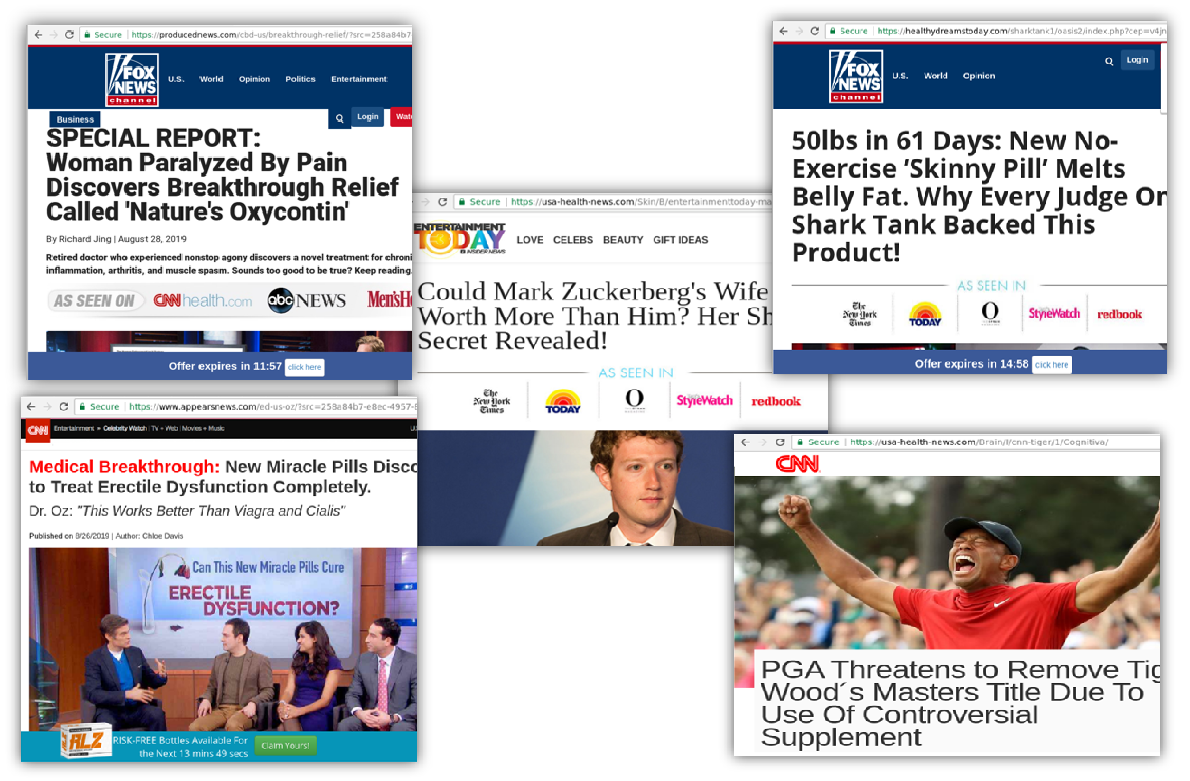
\includegraphics[width=\linewidth]{figs/fake_news.pdf}
        \caption{Example of Phishing on Popular News sites obtained via WPN Ads}
        \label{fake_news}
\end{center}
\end{figure}


\subsection{McAfee Ad Campaign}
This case study is about one of the ad campaigns that we encountered. In this Ad campaign, websites sent ads to the users mentioning that their McAfee antivirus software's license has expired and that they need to renew their McAfee subscription. From our clustering results, we had over 100 advertisements belonging to McAfee ad campaign clustered into a single cluster. This cluster had ads leading users to multiple landing domains. On observing the cluster keenly, we found a few different domains that belong to the same ip address. The cases observed were obtained when \sysname had visited \texttt{https://mogye.info} and \texttt{https://hotmovs.info}. By default, \sysname grants permission to both domains to send notifications. These ads shown by these domains to the user regarding McAfee ad campaign are shown in Fig.\ref{McAfee_case}. After \sysname had clicked these advertisements, these ads had led to domains \texttt{exclusivebreakingstory.com, business-giveaways.com, newtrendingstory.com} and \texttt{hottrendingstory.com}. Moreover, three of these domains resoles to the same IP address '104.238.196.100' and these domains seem to follow a similar pattern. Therefore, we did a reverse-IP lookup on the IP address and found more domains from the same IP address that follow the same pattern. Later, we found that same registrant had registered the discussed 11 domains from the IP address '104.238.191.100'. It has to be noted that none of these landing URLs were accessible later outside it's session. It is interesting to note that domains such as \texttt{healinggreencoffee.com} and \texttt{solutionquotes.com} are involved in this campaign. On trying to find more information on these domains, we found a google result attributing the domain \texttt{healinggreencoffee.com} (refer Fig.\ref{google_res} to a medical news wen page which is another ad campaign that we have observed in our results. Similar to other pages, this page was inaccessible for further enquiry.This search also led us to a report of IP '104.238.196.100' on \texttt{https:/abuseipdb.com} (refer Fig.\ref{ip_report}) which mentioned that the IP was reported over 7 times for phishing, spam and fraud orders. 

\begin{figure}[ht]
\begin{center}
 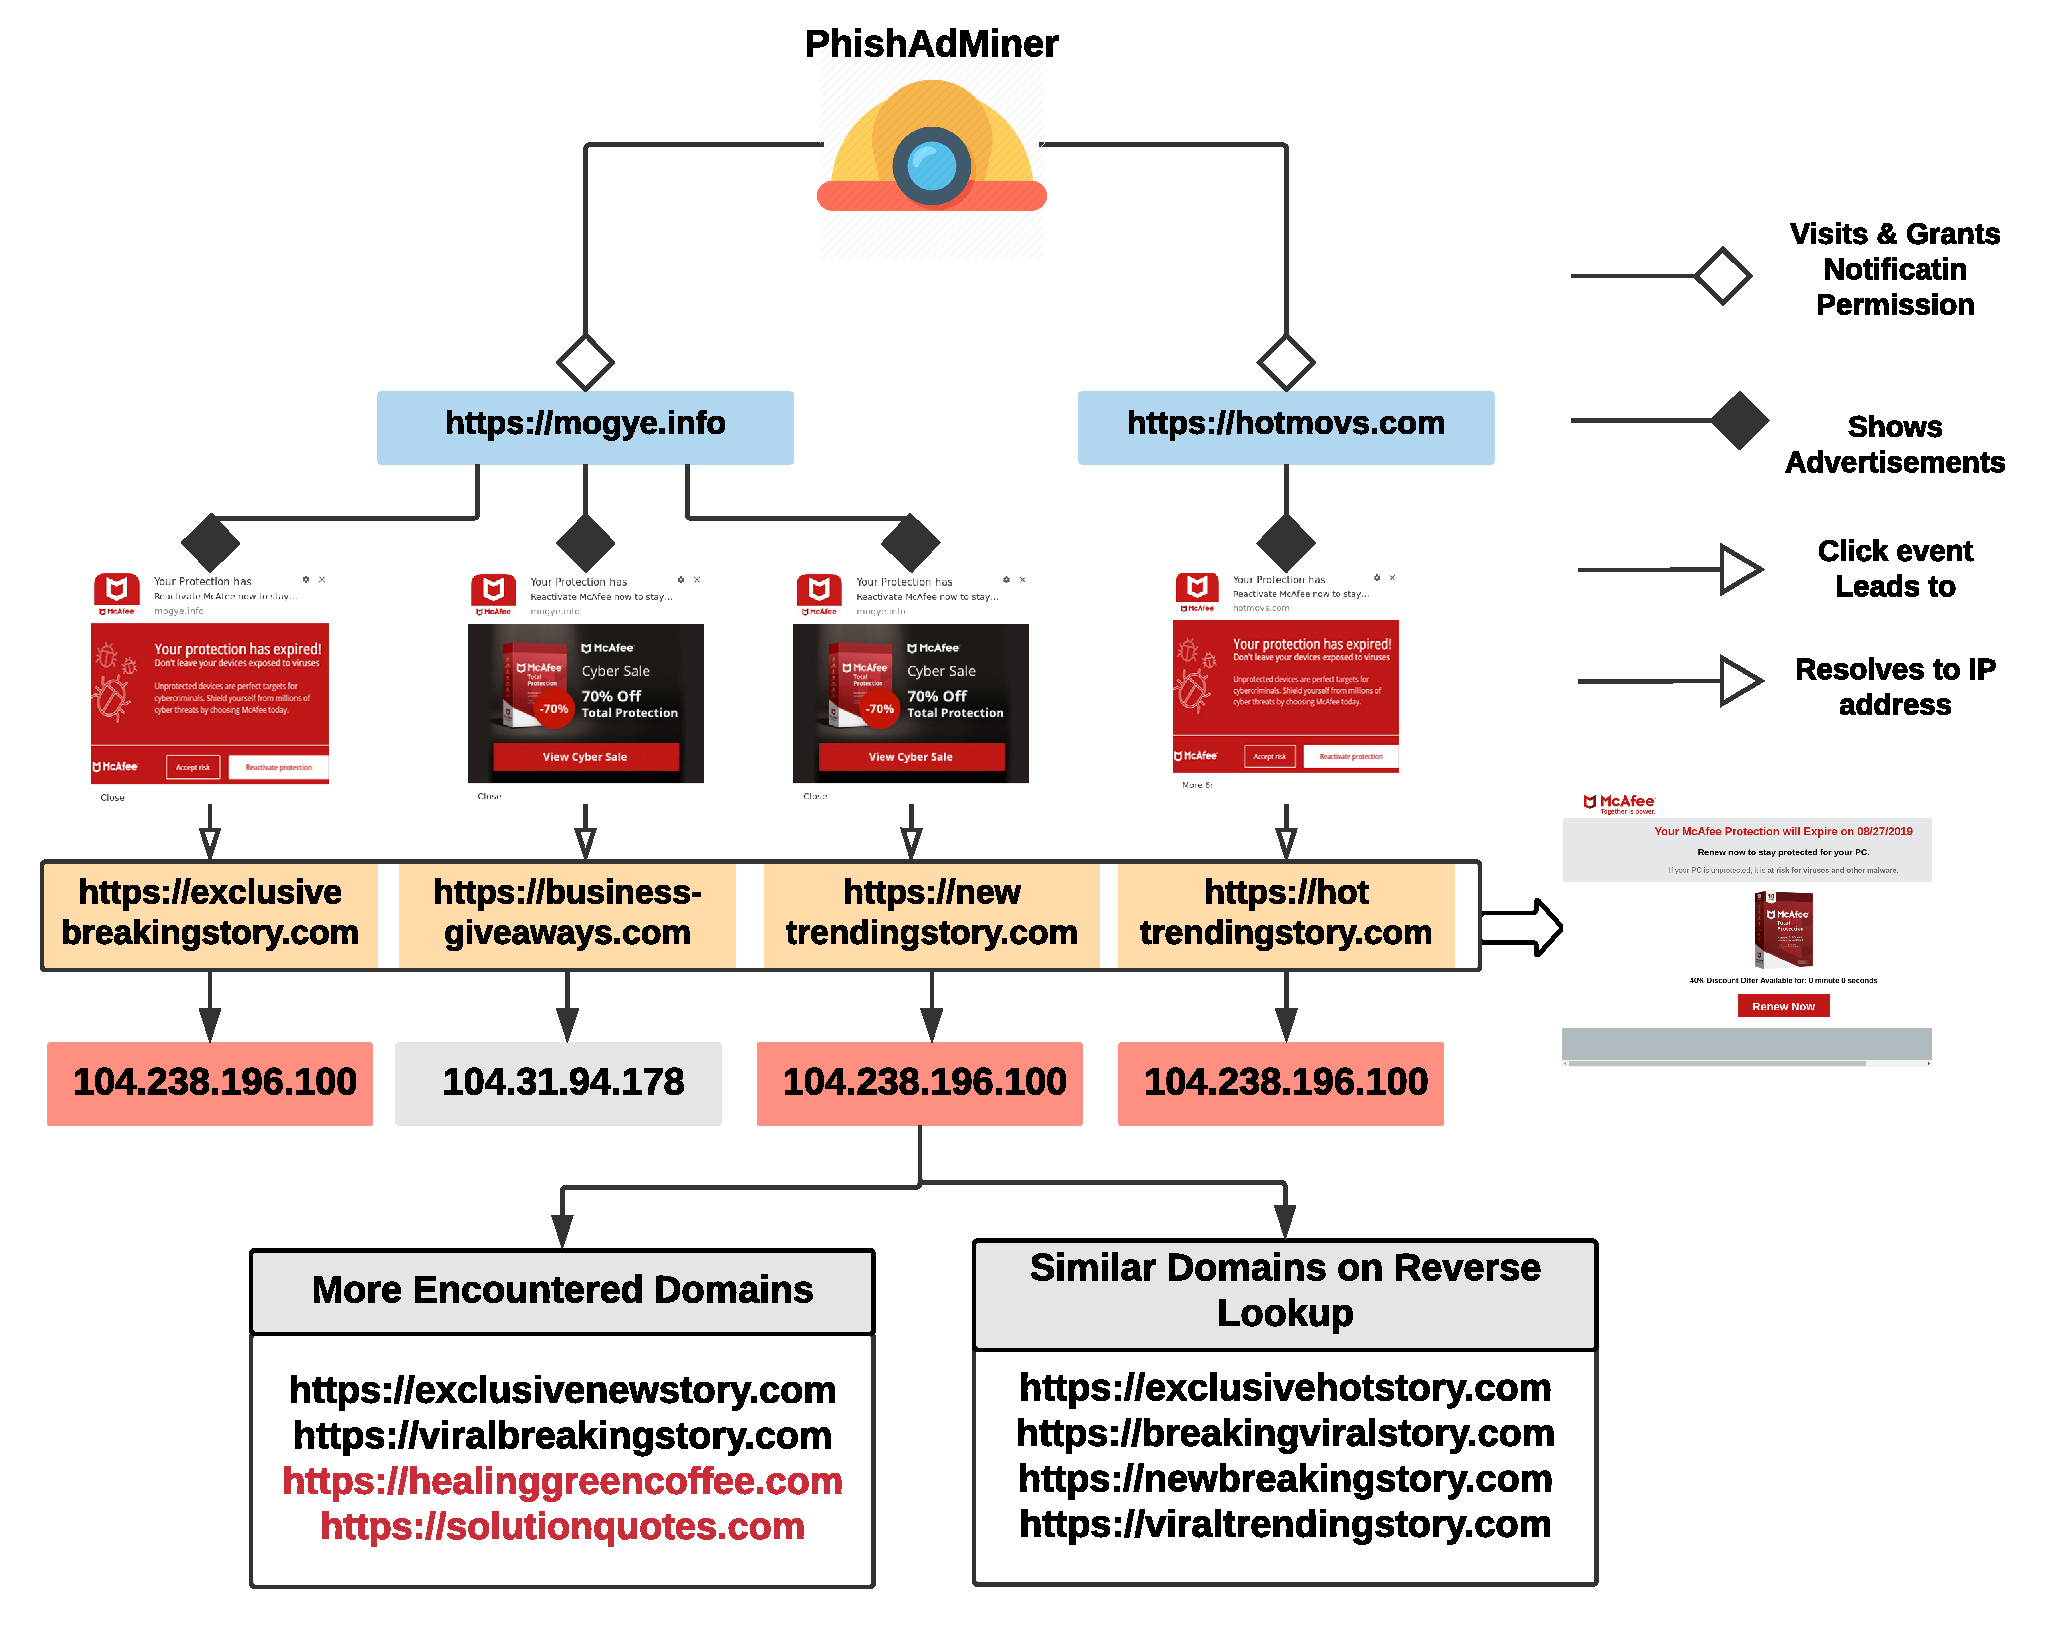
\includegraphics[width=\linewidth]{figs/mcafee_case2.pdf}
        \caption{Case study on McAfee Ad Campaign}
        \label{McAfee_case}
\end{center}
\begin{center}
 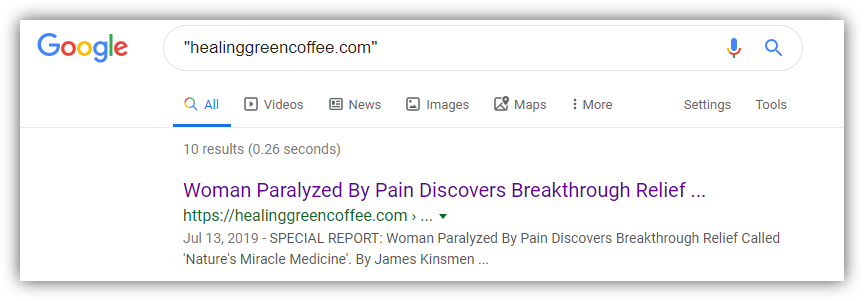
\includegraphics[width=\linewidth]{figs/healinggreencoffee.png}
        \caption{Searh Result on the domain 'healinggreencoffee.com'}
        \label{google_res}
\end{center}
\begin{center}
 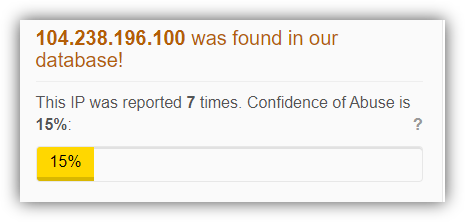
\includegraphics[width=\linewidth]{figs/ip_report.png}
        \caption{Report on the IP '104.238.196.100'}
        \label{ip_report}
\end{center}
\end{figure}

Considering this case is suspicious enough, we follow to check on the other domain that belongs to this cluster \texttt{business-giveaways.com}. Although, we couldn't decide on it's maliciousness by visiting the landing page, on obtaining the registrant information from WHOIS domain, we found that this domain belongs to the same individuals who had registered the domains \texttt{usa-health-news.com, appearsnews.com, healthydreamstoday.com} that were discussed in the previous case study. Based on the fact that, the domians from previous case study served fake news via phishing and the current domain 'business-giveaways.com' as well is registered from the same individual, we tag 'business-giveaways.com' as suspicious/malicious domain. Therefore, our clustering proved to be an efficient way to identify similar ad campaigns and discover similar cases effectively.


%%%%%%%%%%%%%%%%%%%%%%%%
\subsection{Mobile targeted click-bait}
In this section, we discuss cases that were tailored to specifically target mobile users into clicking the notification. In Mobile environment, we encountered a lot of ads that are fake 'Missed Call' messages. Few of such advertisements are shown in Fig. \ref{fig:mobile_disguised_notification}. Note that in Fig. \ref{fig:mobile_disguised_notification}(b), the third notification is a fake Amber Alert with the city name of the test device we have. Because website server can get visitor's IP address, it is fairly easy to the obtain the geographic location of that IP address. By doing so, the fake notification would appear more legitimately to the users. Further, we analyzed one of the cases manually to figure out the motive behind such advertisements. The case that we analyzed in detail is portrayed in Fig. \ref{fig:mobile}. In this example, the ad shows '1 Missed Call' message. When an user clicks on it, it first lands in a web page saying "You will lose 14kg in 28 days.". Then after a few seconds, it automatically redirects to a page selling the drug. To urge the users into buying the drug before the offer expires or before the drug is unavailable, the page displays a countdown for 3 minutes. Once the user agrees to buy the drug, the website composes several forms, aiming at collecting sensitive information like phone number, email address and contact address. As it can be observed from Fig. \ref{fig:mobile_disguised_notification}(a), when there appear a large number of notifications, information regarding the sender application and domain name are hidden to make space for new notifications\samuel{I'm not quite sure what this means. I can still see "chromium" and domain names in the notification. If the user wants to click the notification below, he needs to scroll up and expand those notifications. At that time, the app name and domain name will be shown.}. This proves to be significant way for scammers to trick mobile users and can lead to potential loss of significant information for the users.

% The case in Fig. \ref{fig:mobile} is an example of mobile specific click-bait. The notification will be disguised as other application's notification and lure users to click, in this case, it first lands in a web page saying "You will lose 14kg in 28 days.". Then after a few seconds, it redirects itself to a page selling the drug. To make users feel urgent and purchase the drug fast without thinking it through, it even puts a 3 minutes countdown. Then after this point, the website composes several forms, aiming at collecting sensitive information like phone number and email address. There are more examples shown in Fig. \ref{fig:mobile_disguised_notification}. Noted that in Fig. \ref{fig:location}, the third notification is a fake Amber Alert with the city name of out test device. Because website server can get visitor' IP address, it is fairly easy to the obtain the geographic location of that IP address. By doing so, the fake notification would be more appealing.


\begin{figure}[h]
\begin{center}
    \begin{subfigure}{.2\textwidth} 
    \begin{center}
        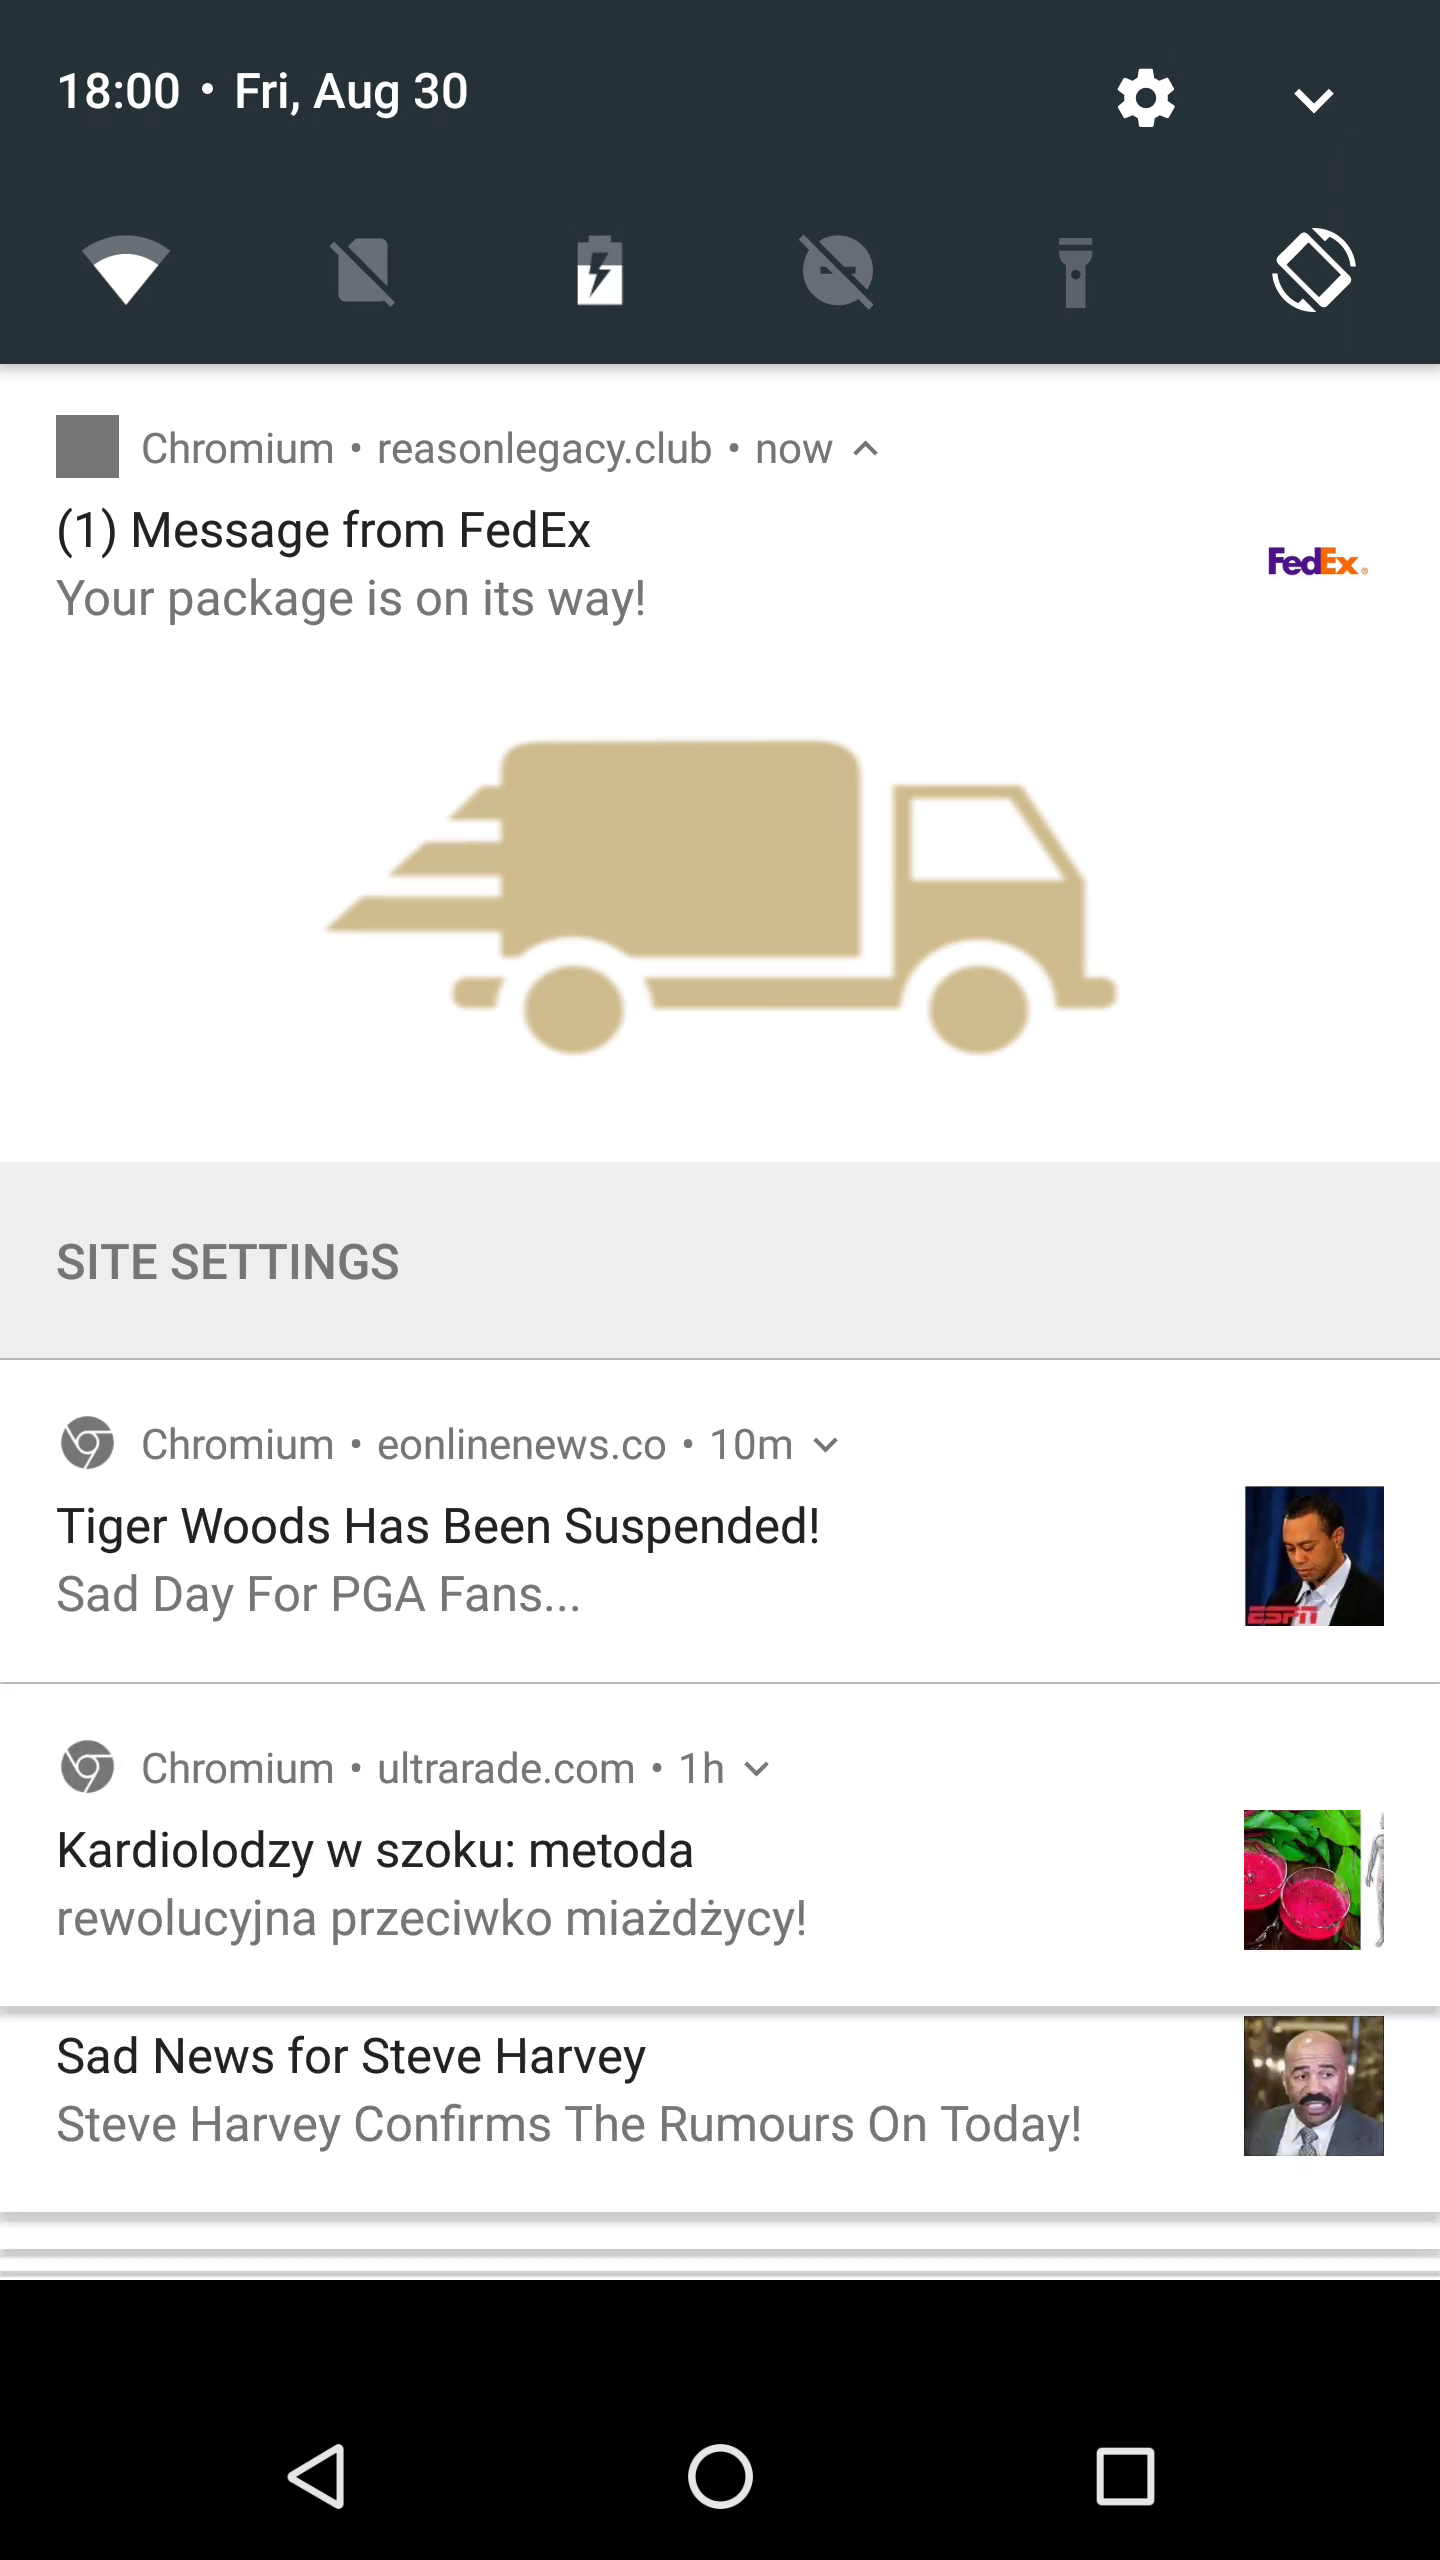
\includegraphics[width=\linewidth]{figs/mobile_disguised_2}
        \caption{}
    \end{center}
    \end{subfigure}
    \begin{subfigure}{.2\textwidth} 
    \begin{center}
        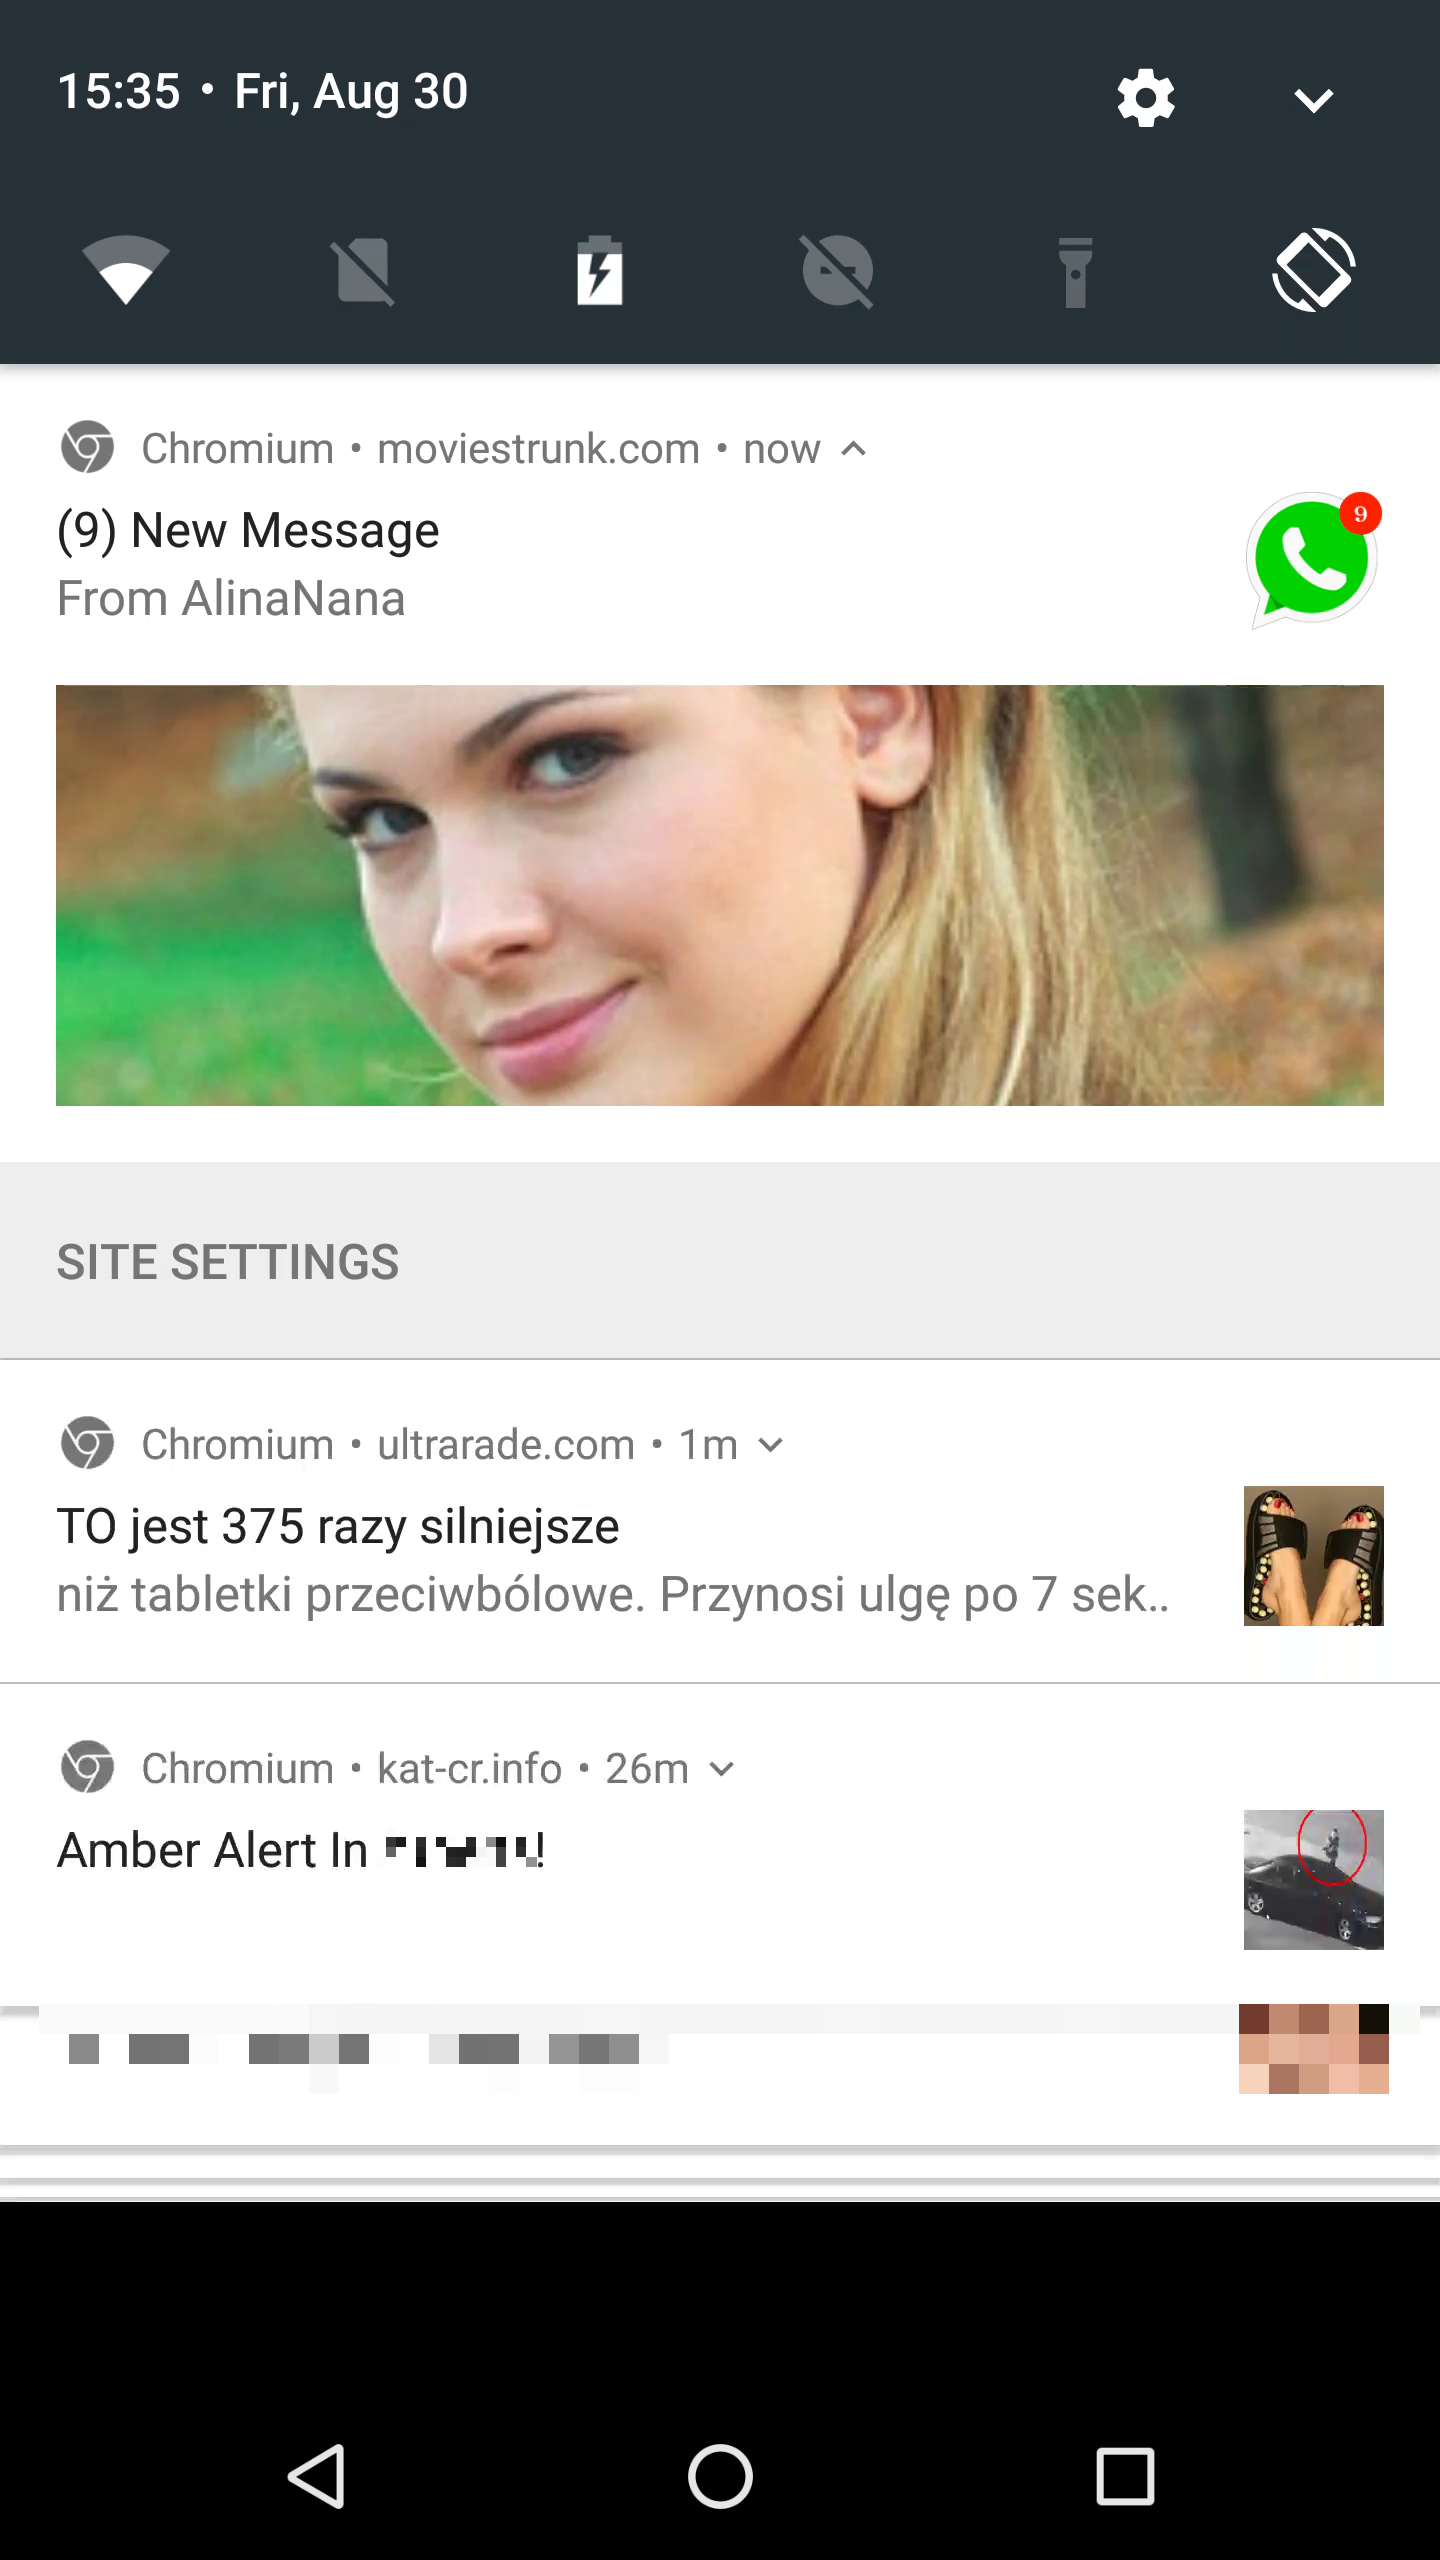
\includegraphics[width=\linewidth]{figs/mobile_disguised_3}
        \caption{}
        \label{fig:location}
    \end{center}
    \end{subfigure}
    \caption{Click-Bait Examples on Mobile: (a)Ad disguised as Fedex app's notification (b)Ad disguised as WhatsApp's notification}
    \label{fig:mobile_disguised_notification}
\end{center}
\end{figure}


\begin{figure*}[h]
\begin{center}
    \begin{subfigure}{.18\textwidth}
    \begin{center}
        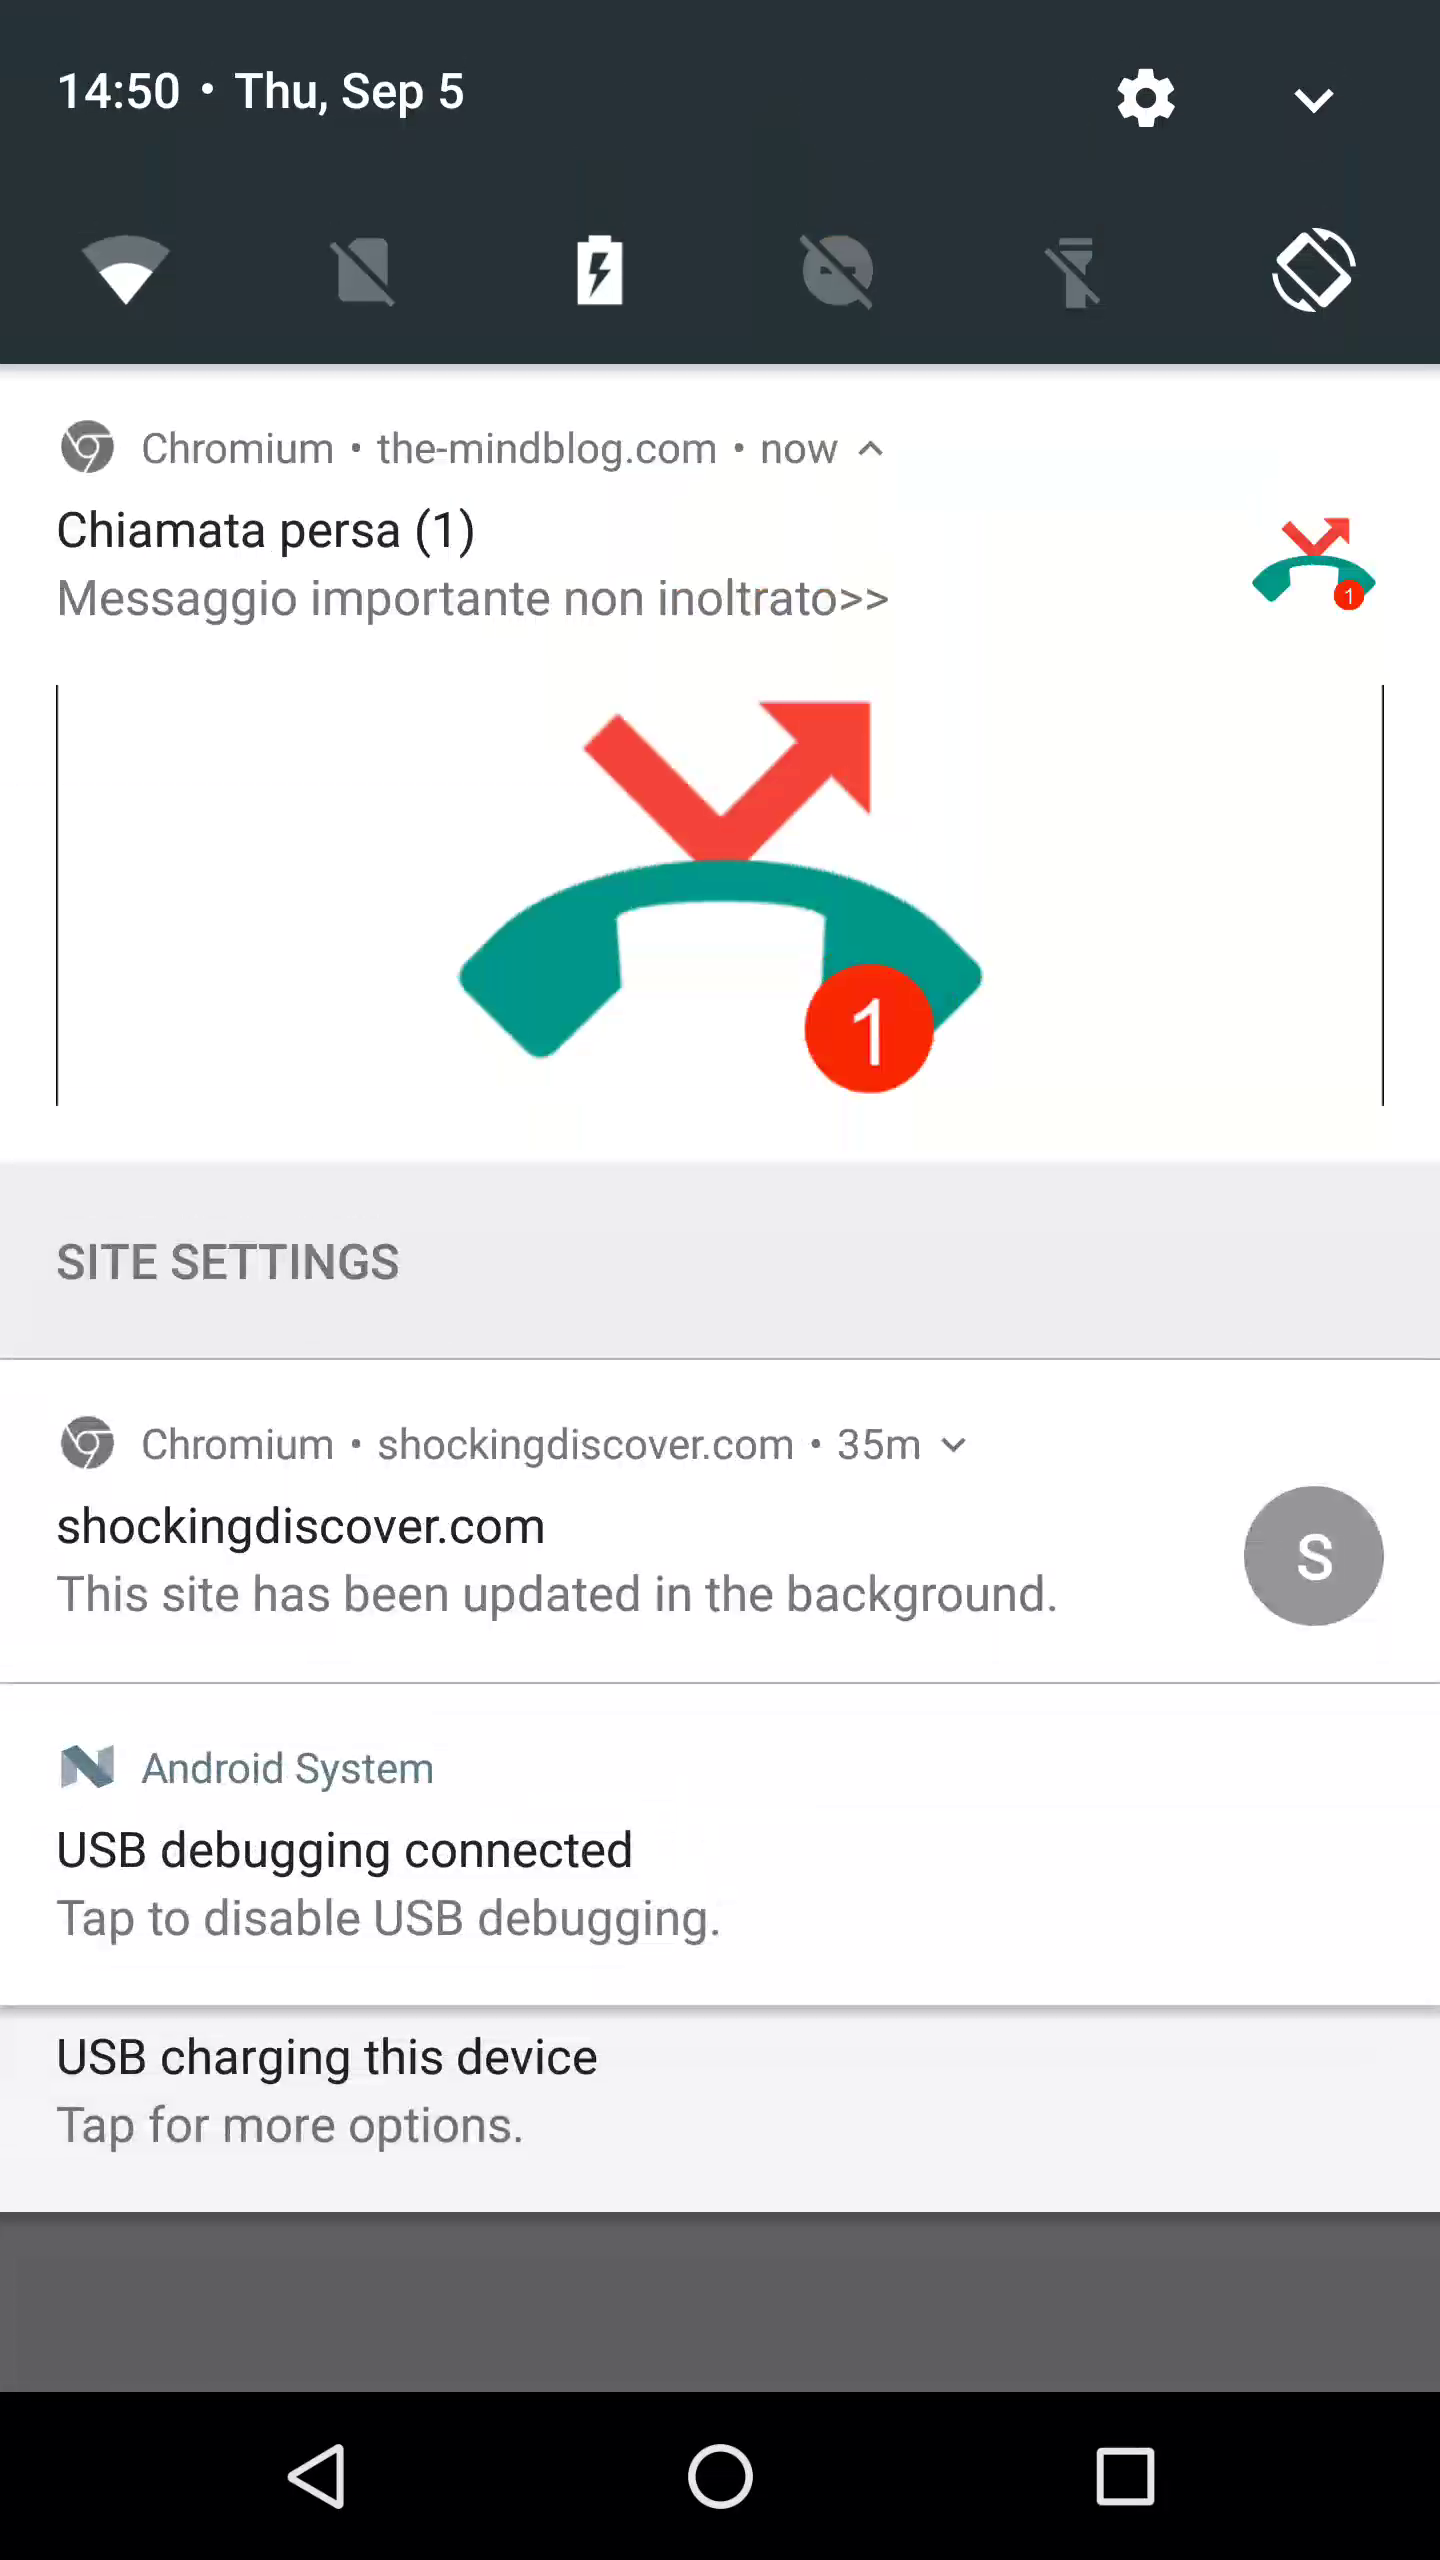
\includegraphics[scale=0.06]{figs/mobile_1}
        \caption{}
    \end{center}
    \end{subfigure}
   \begin{subfigure}{.18\textwidth} 
    \begin{center}
        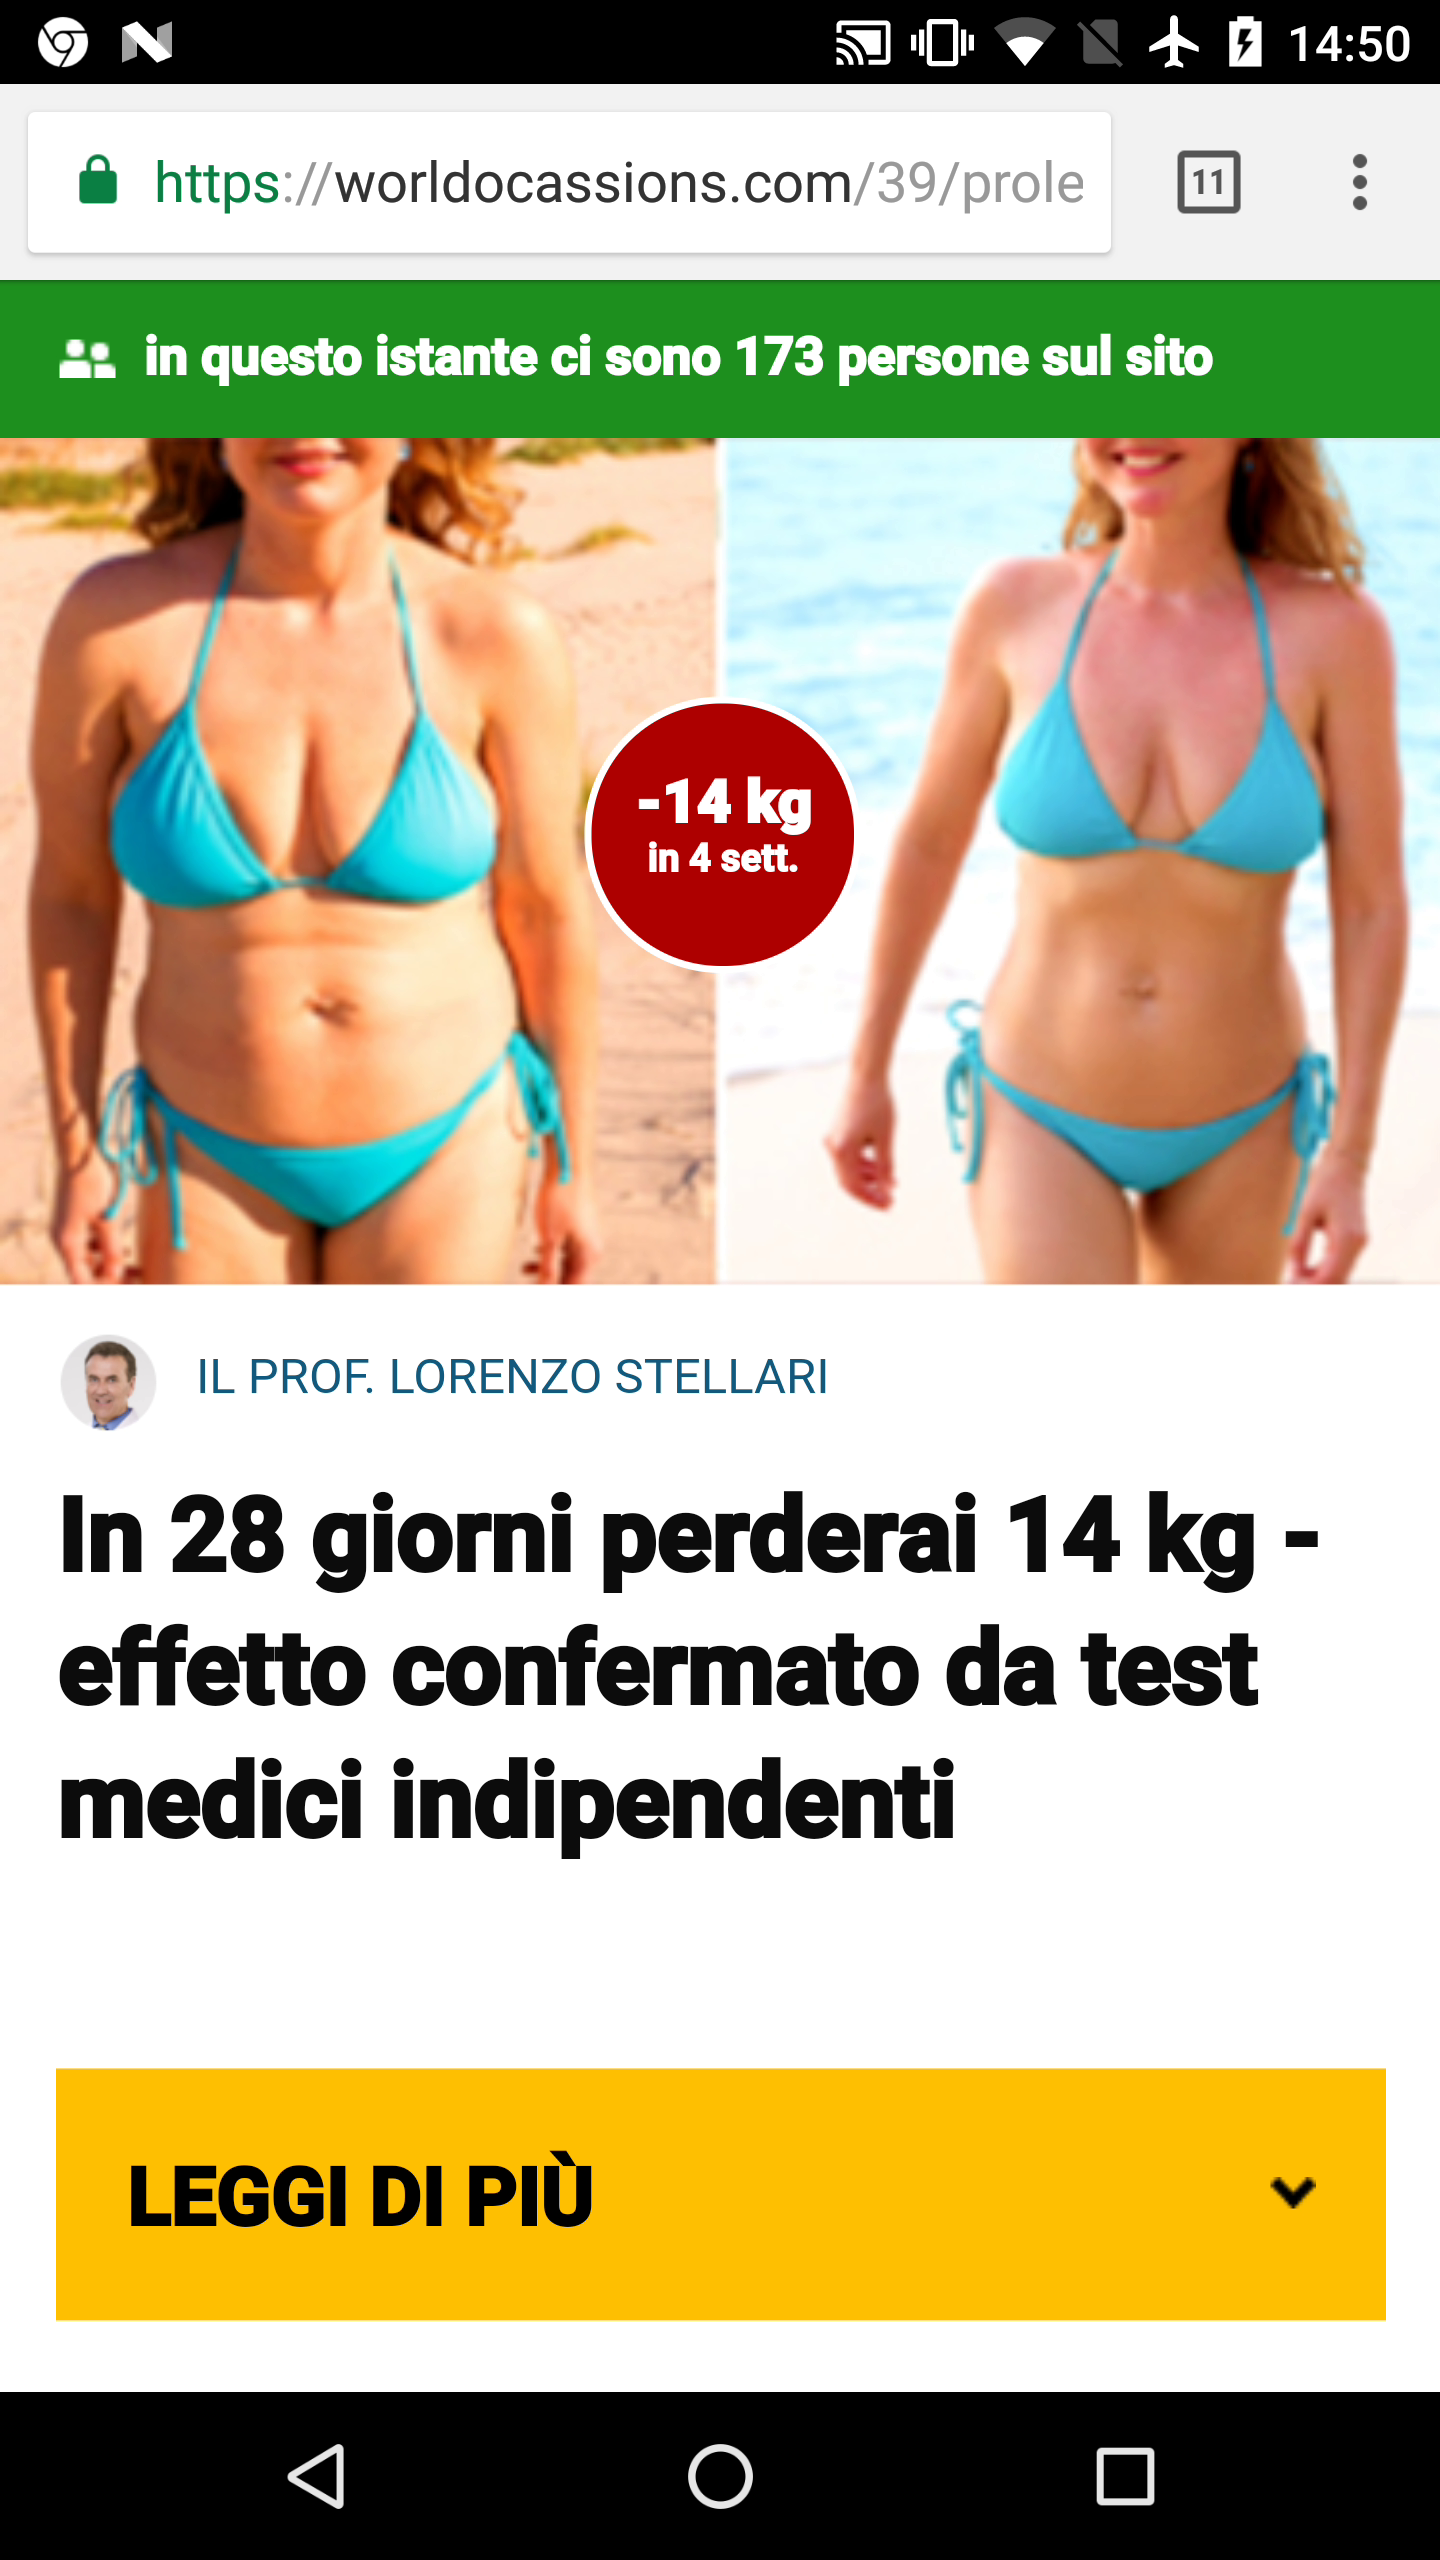
\includegraphics[scale=0.06]{figs/mobile_2}
        \caption{}
    \end{center}
    \end{subfigure}
    \begin{subfigure}{.18\textwidth}
    \begin{center}
        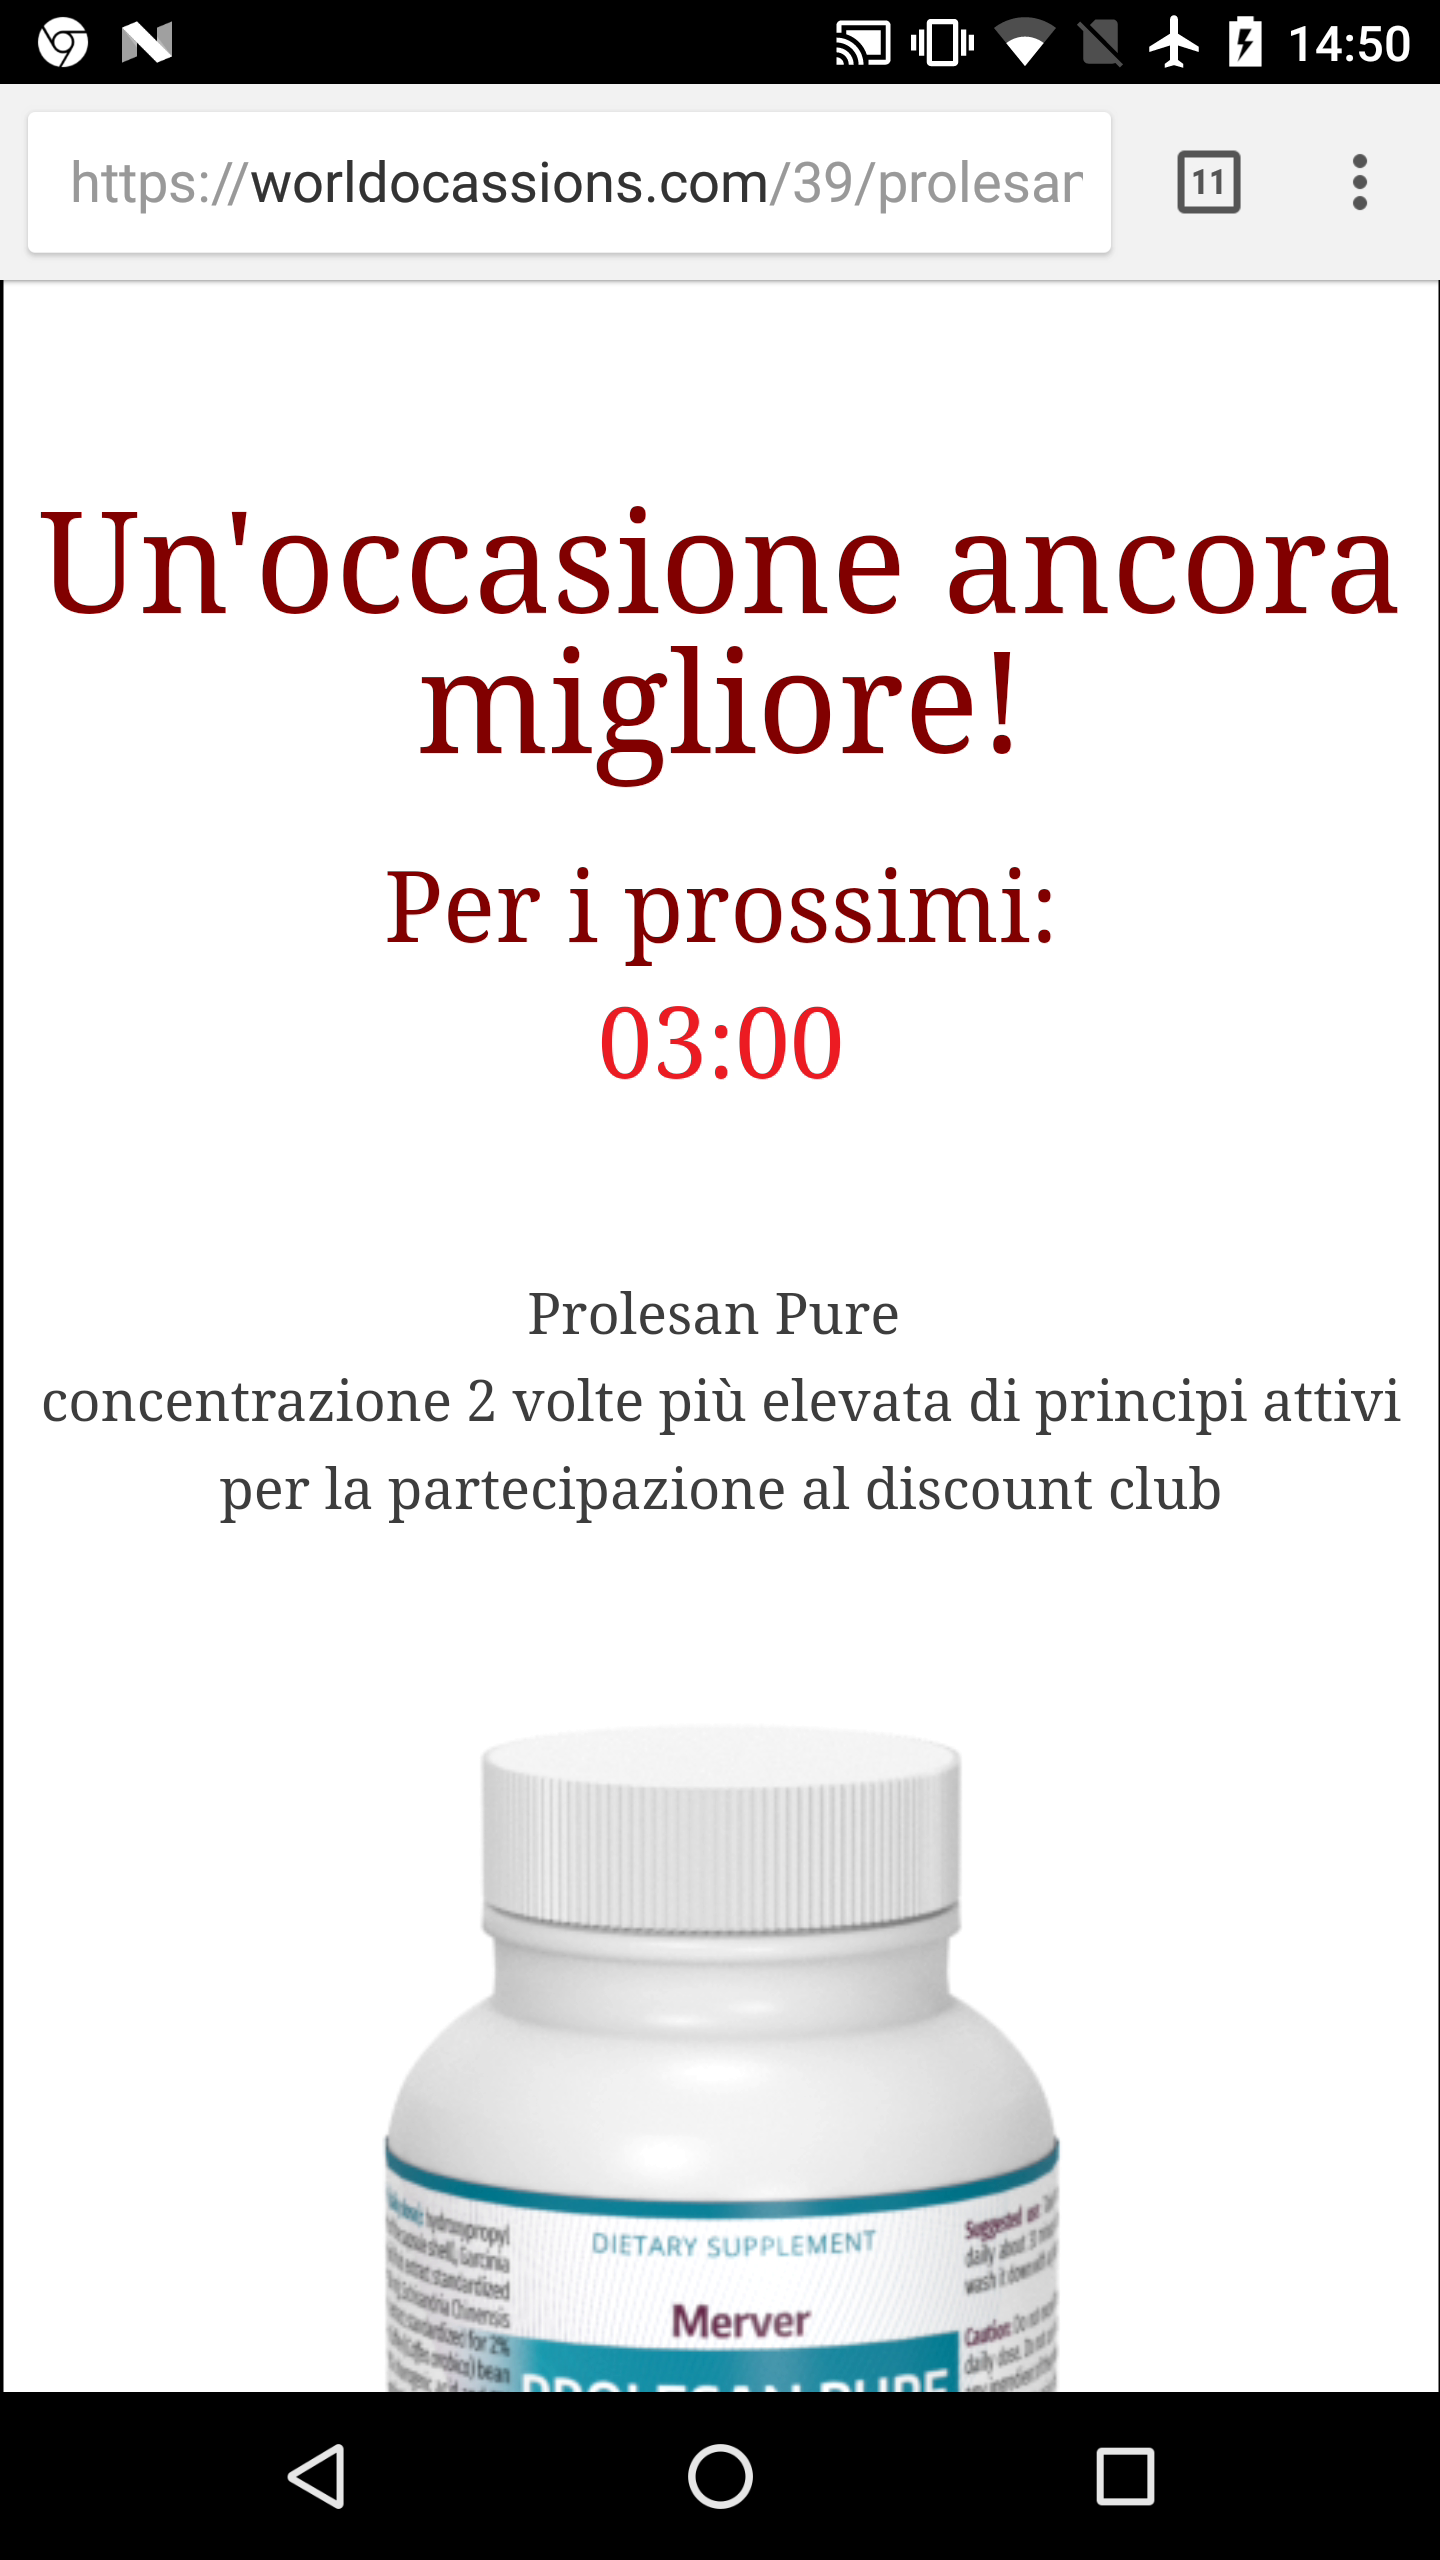
\includegraphics[scale=0.06]{figs/mobile_3}
        \caption{}
    \end{center}
    \end{subfigure}
    \begin{subfigure}{.18\textwidth}
    \begin{center}
        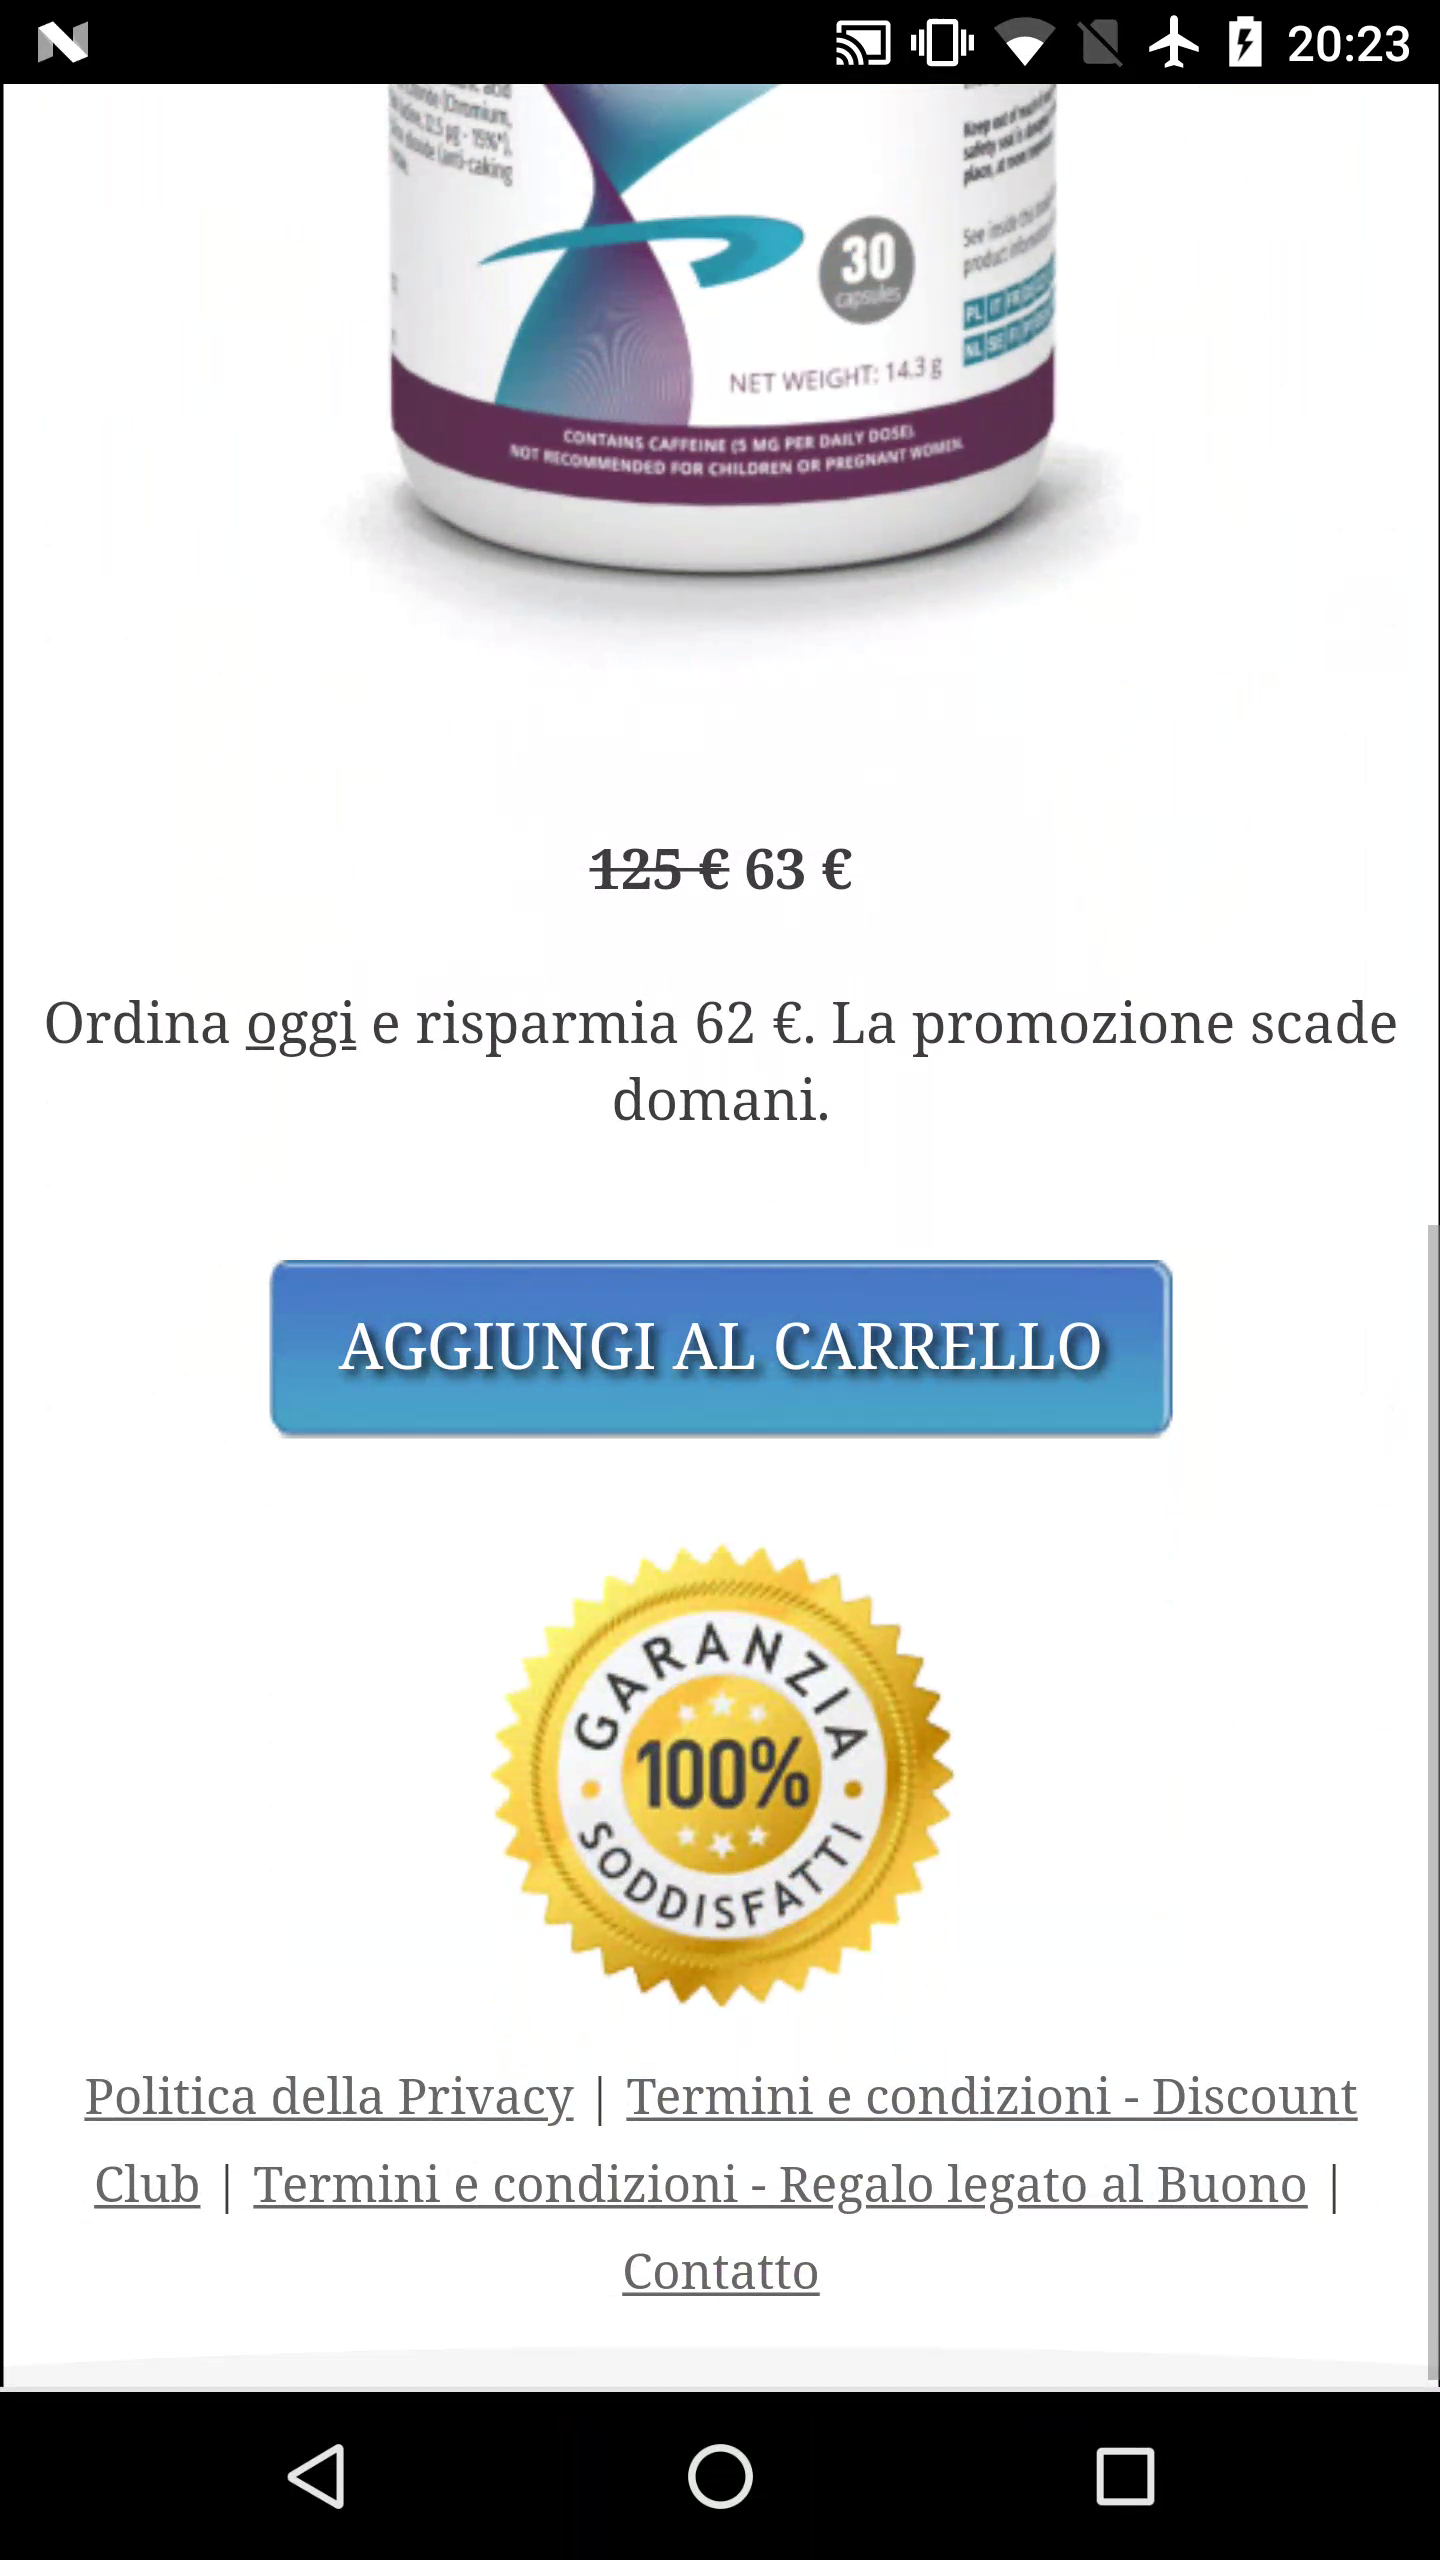
\includegraphics[scale=0.06]{figs/mobile_4}
        \caption{}
    \end{center}
    \end{subfigure}
    \begin{subfigure}{.18\textwidth} 
    \begin{center}
        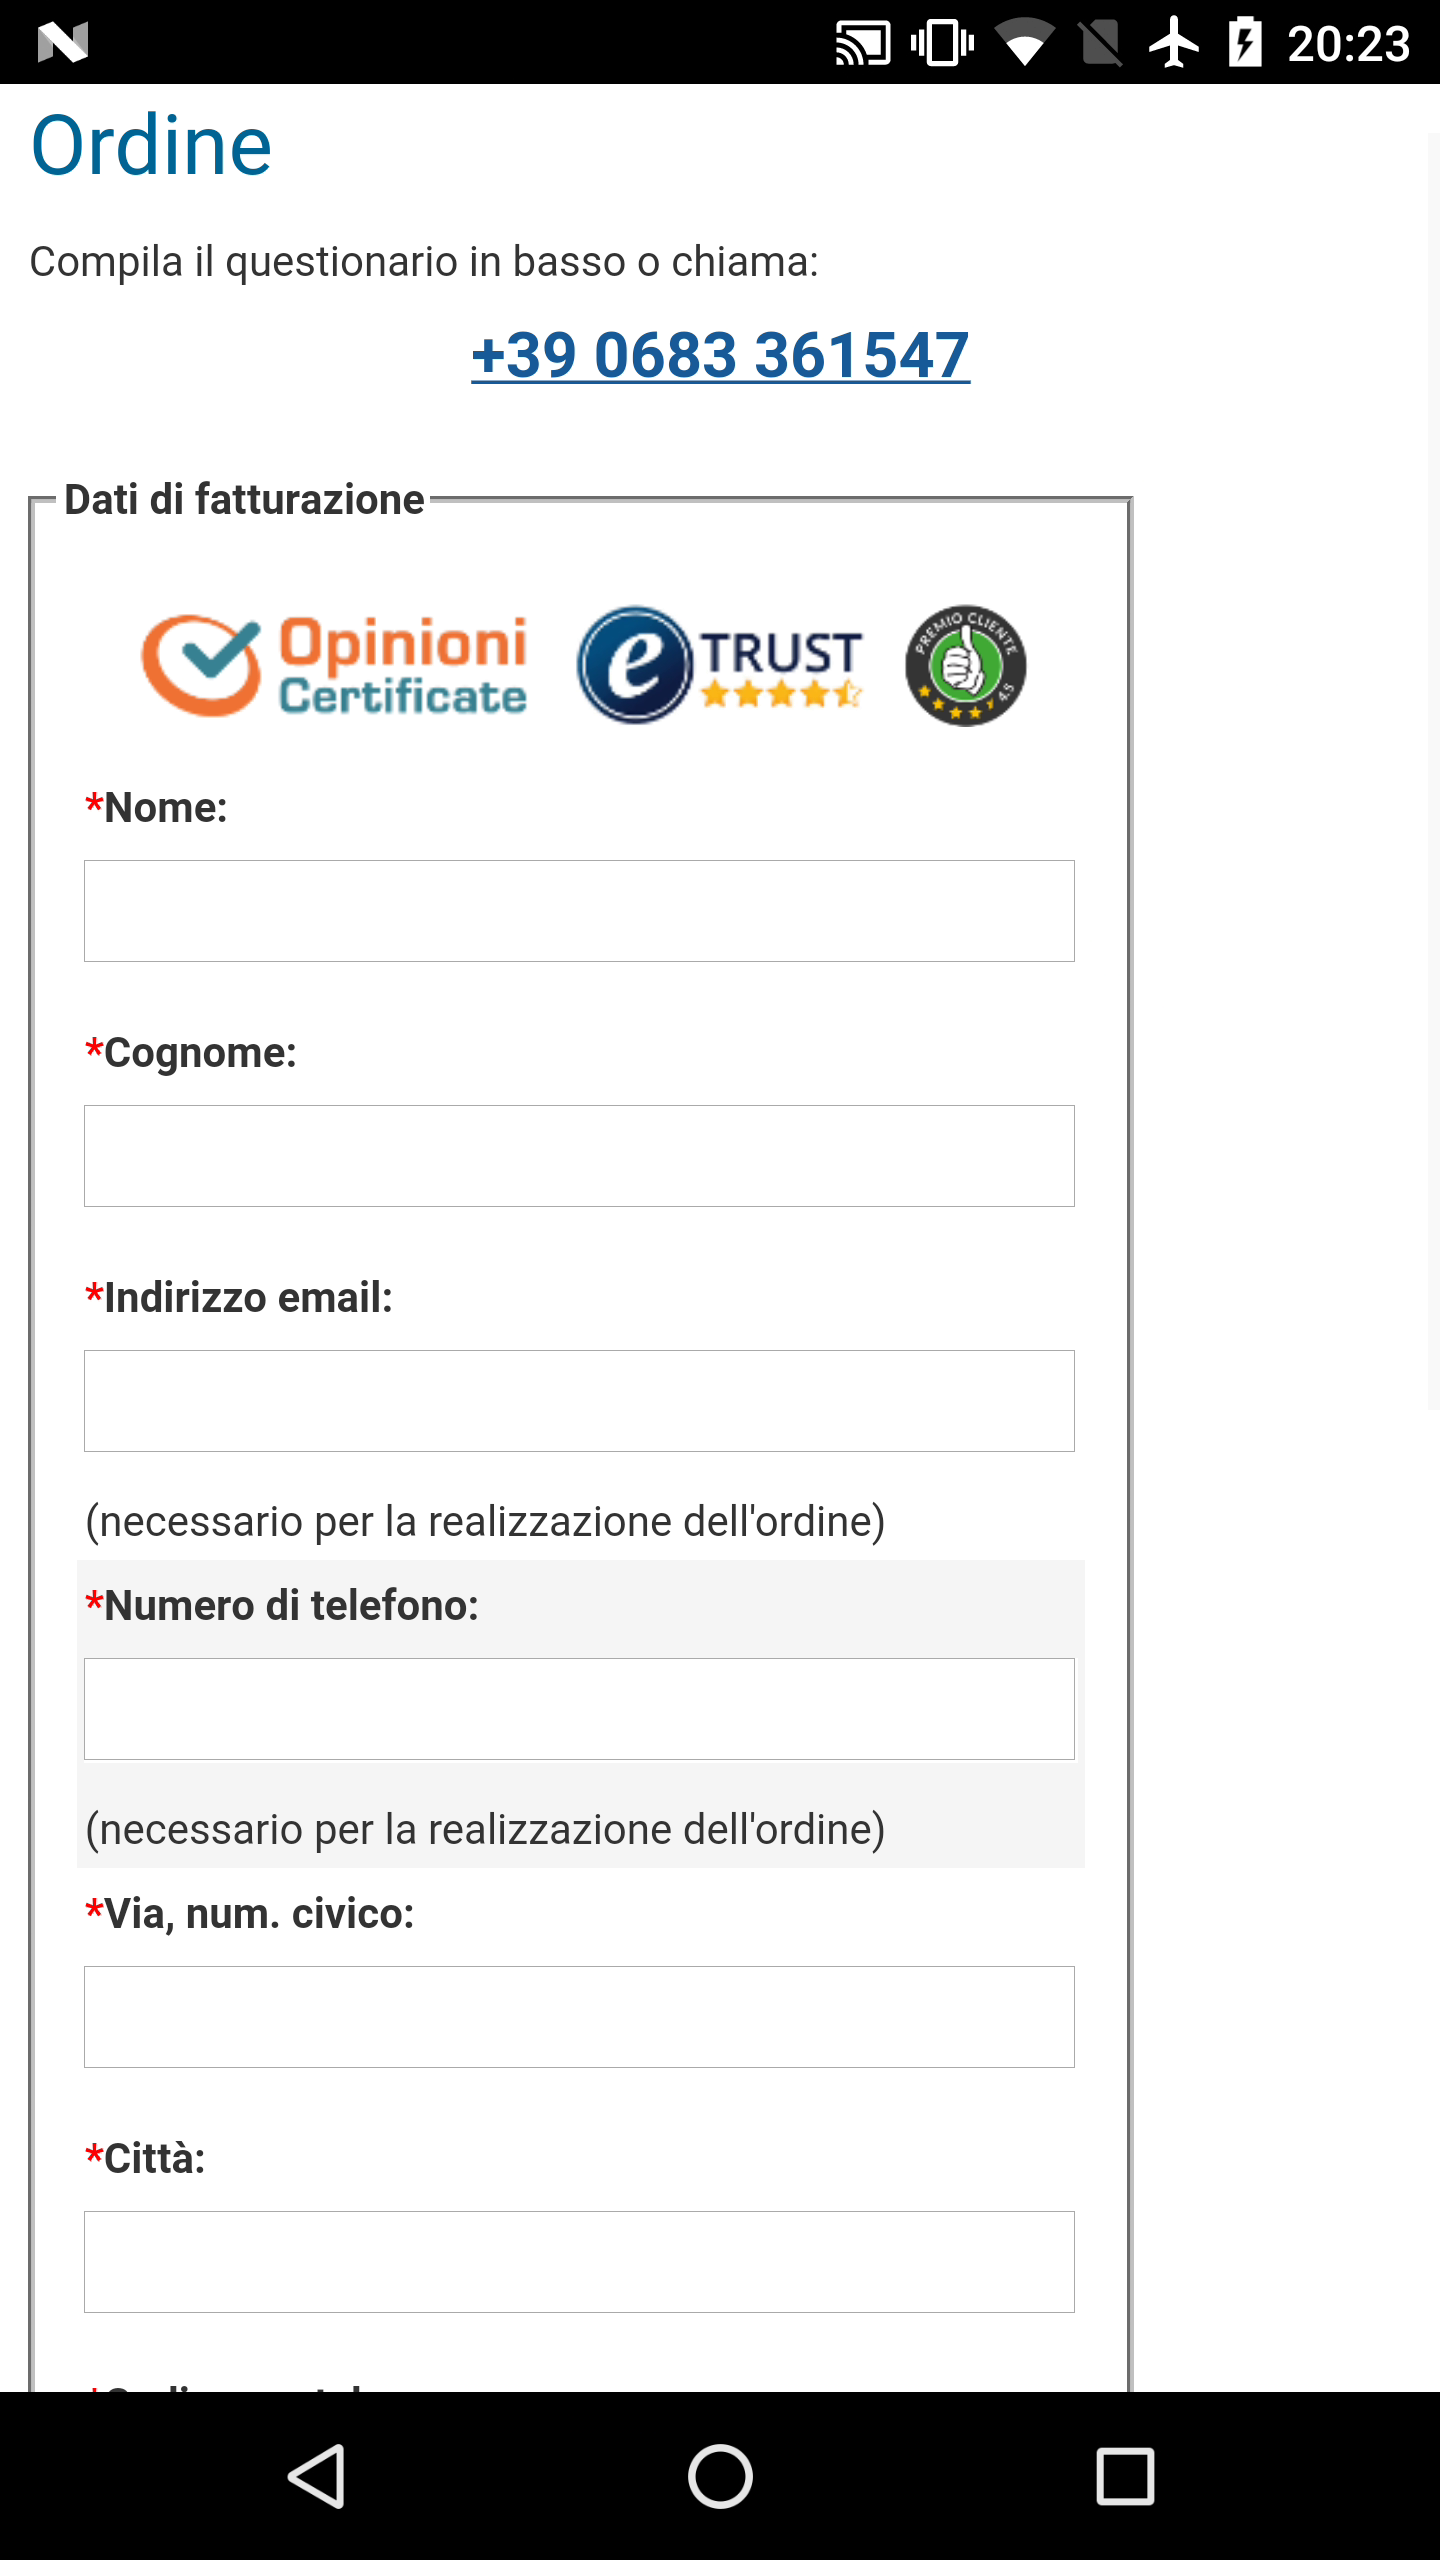
\includegraphics[scale=0.06]{figs/mobile_5}
        \caption{}
    \end{center}
    \end{subfigure}
    
    \caption{Mobile Case Study (a)Displays Notification of a 'Missed Call' (b)Initial Landing Page after clicking the notification displays article on weight loss (c) Redirected Page (d) Redirected Page-contd. (e)Displays a form collecting sensitive information }
    \label{fig:mobile}
\end{center}
\end{figure*}



% \begin{figure}[h]
% \begin{center}
%     \begin{subfigure}{.24\textwidth}
%     \begin{center}
%         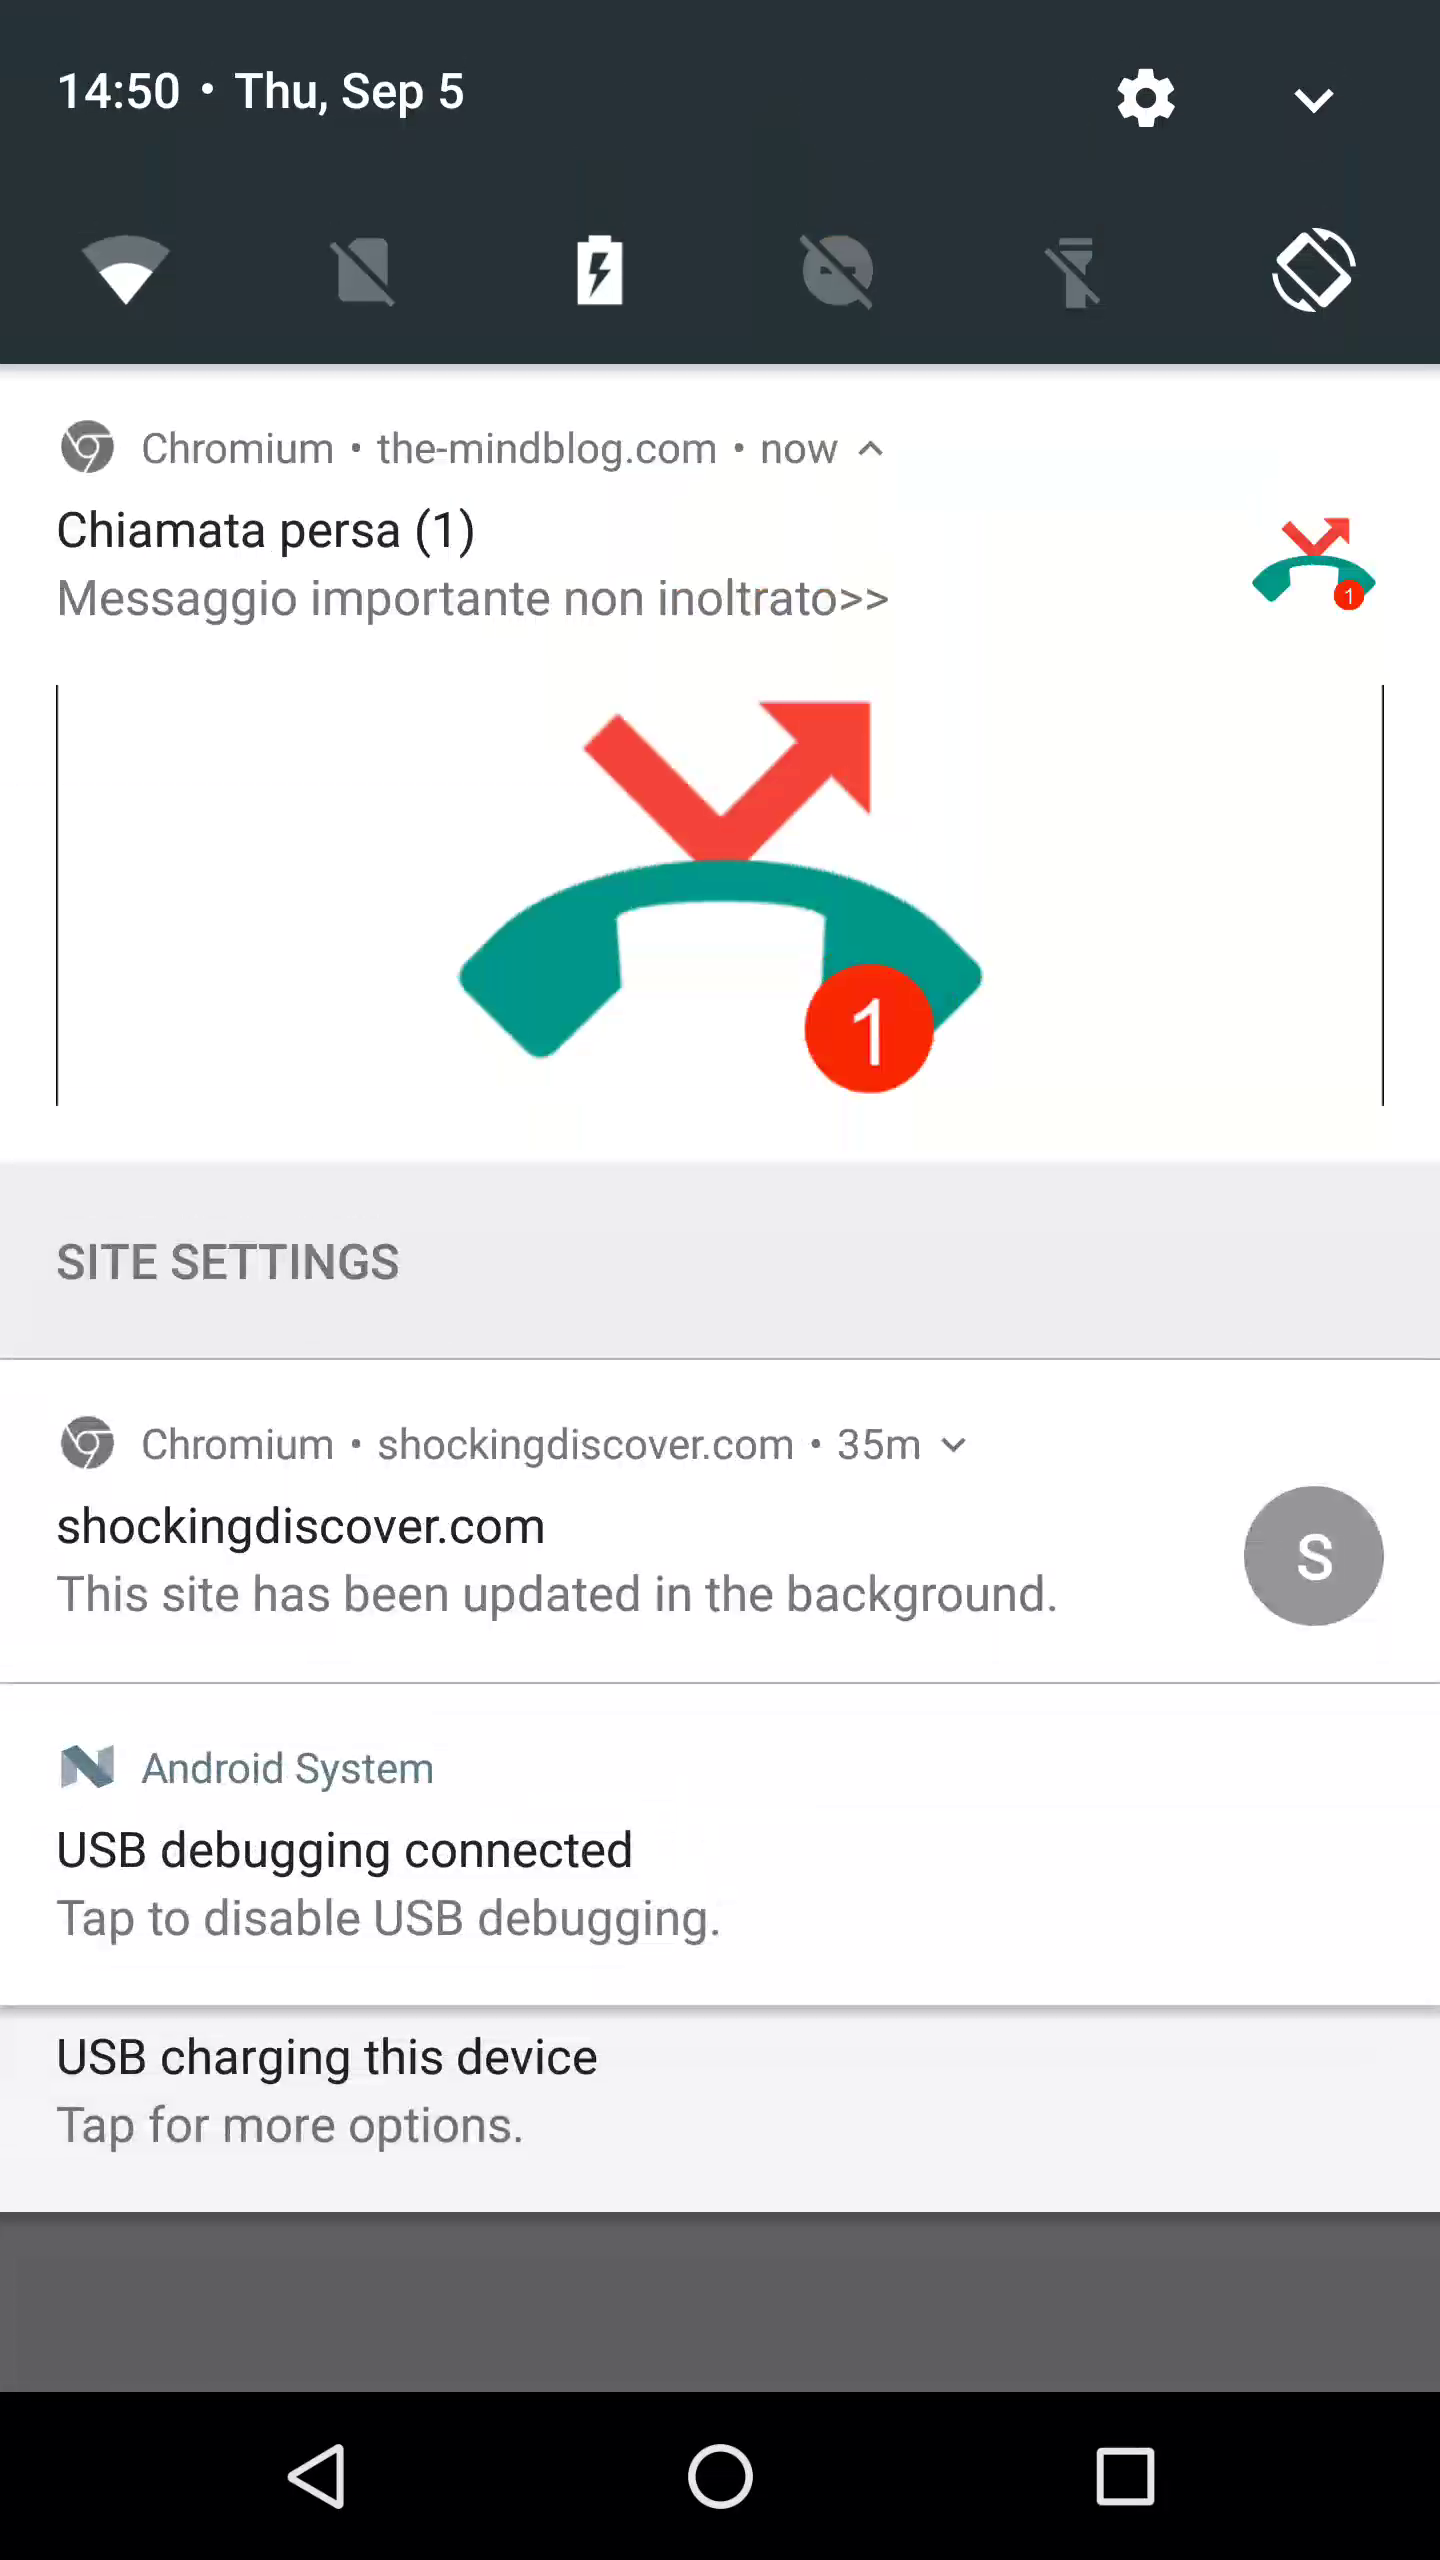
\includegraphics[scale=0.08]{figs/mobile_1}
%         \caption{Notification}
%     \end{center}
%     \end{subfigure}
%     \begin{subfigure}{.24\textwidth} 
%     \begin{center}
%         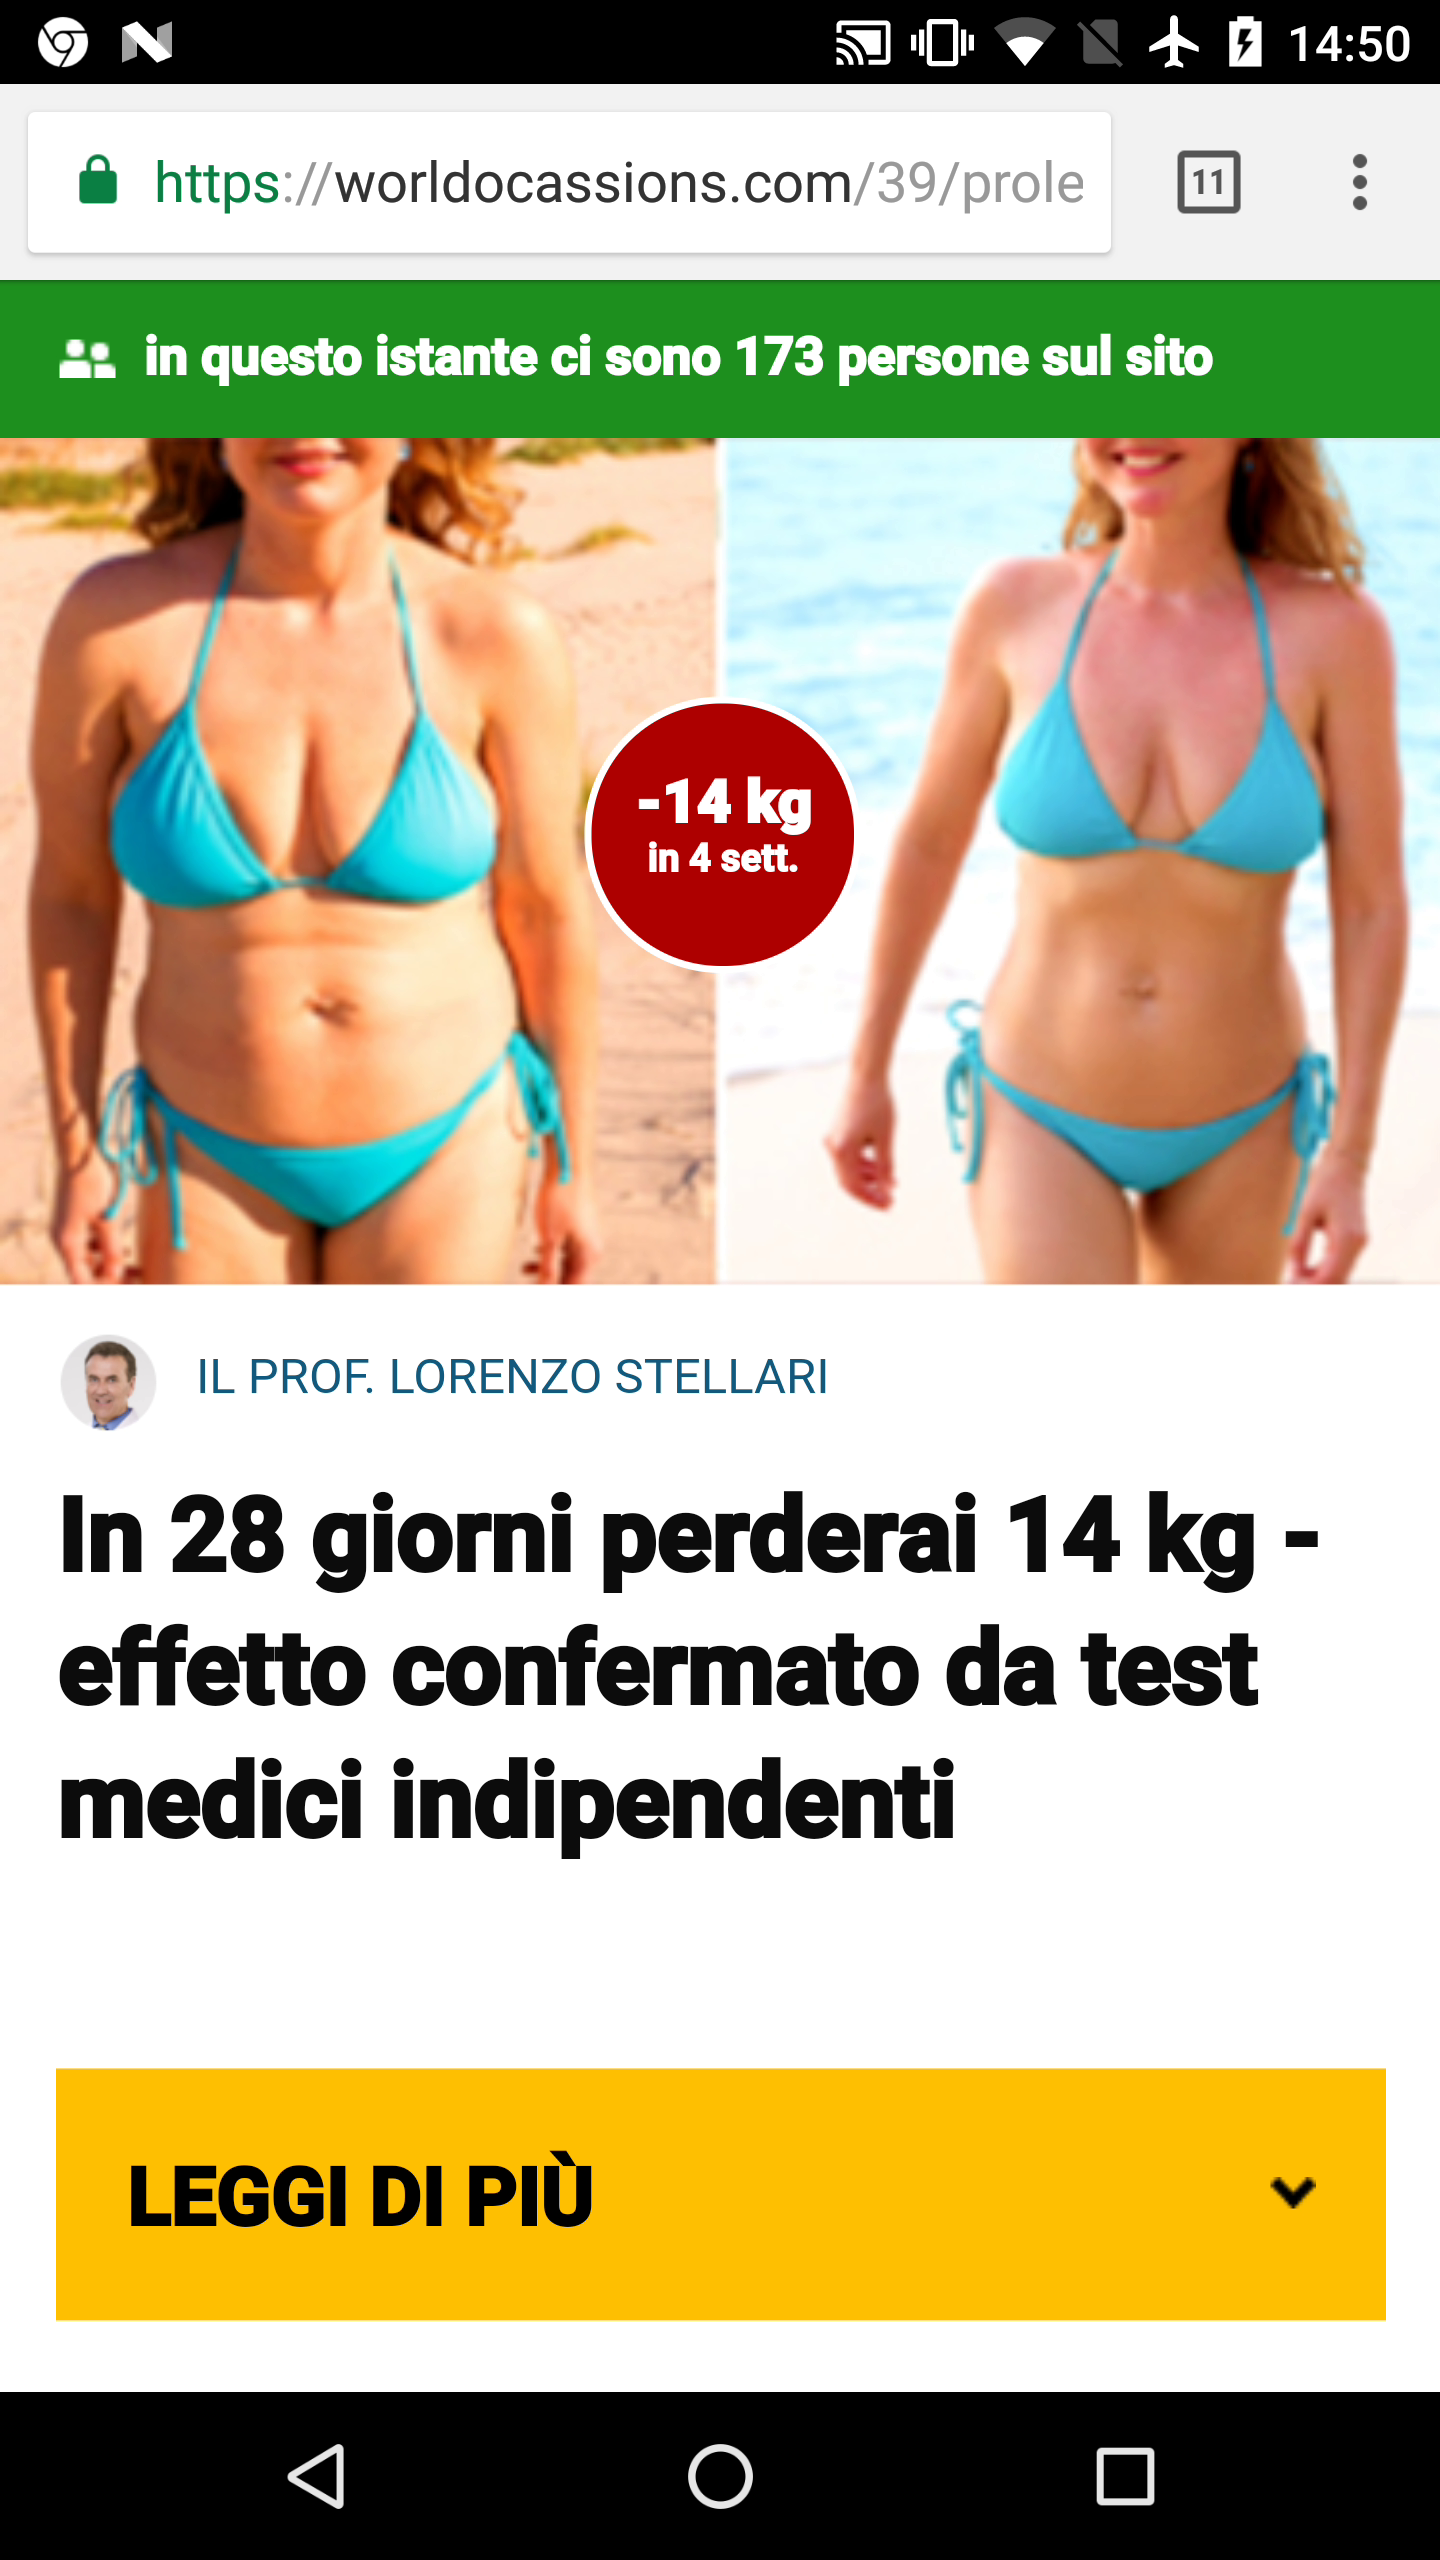
\includegraphics[scale=0.08]{figs/mobile_2}
%         \caption{Initial Landing Page}
%     \end{center}
%     \end{subfigure}
%     \begin{subfigure}{.24\textwidth} 
%     \begin{center}
%         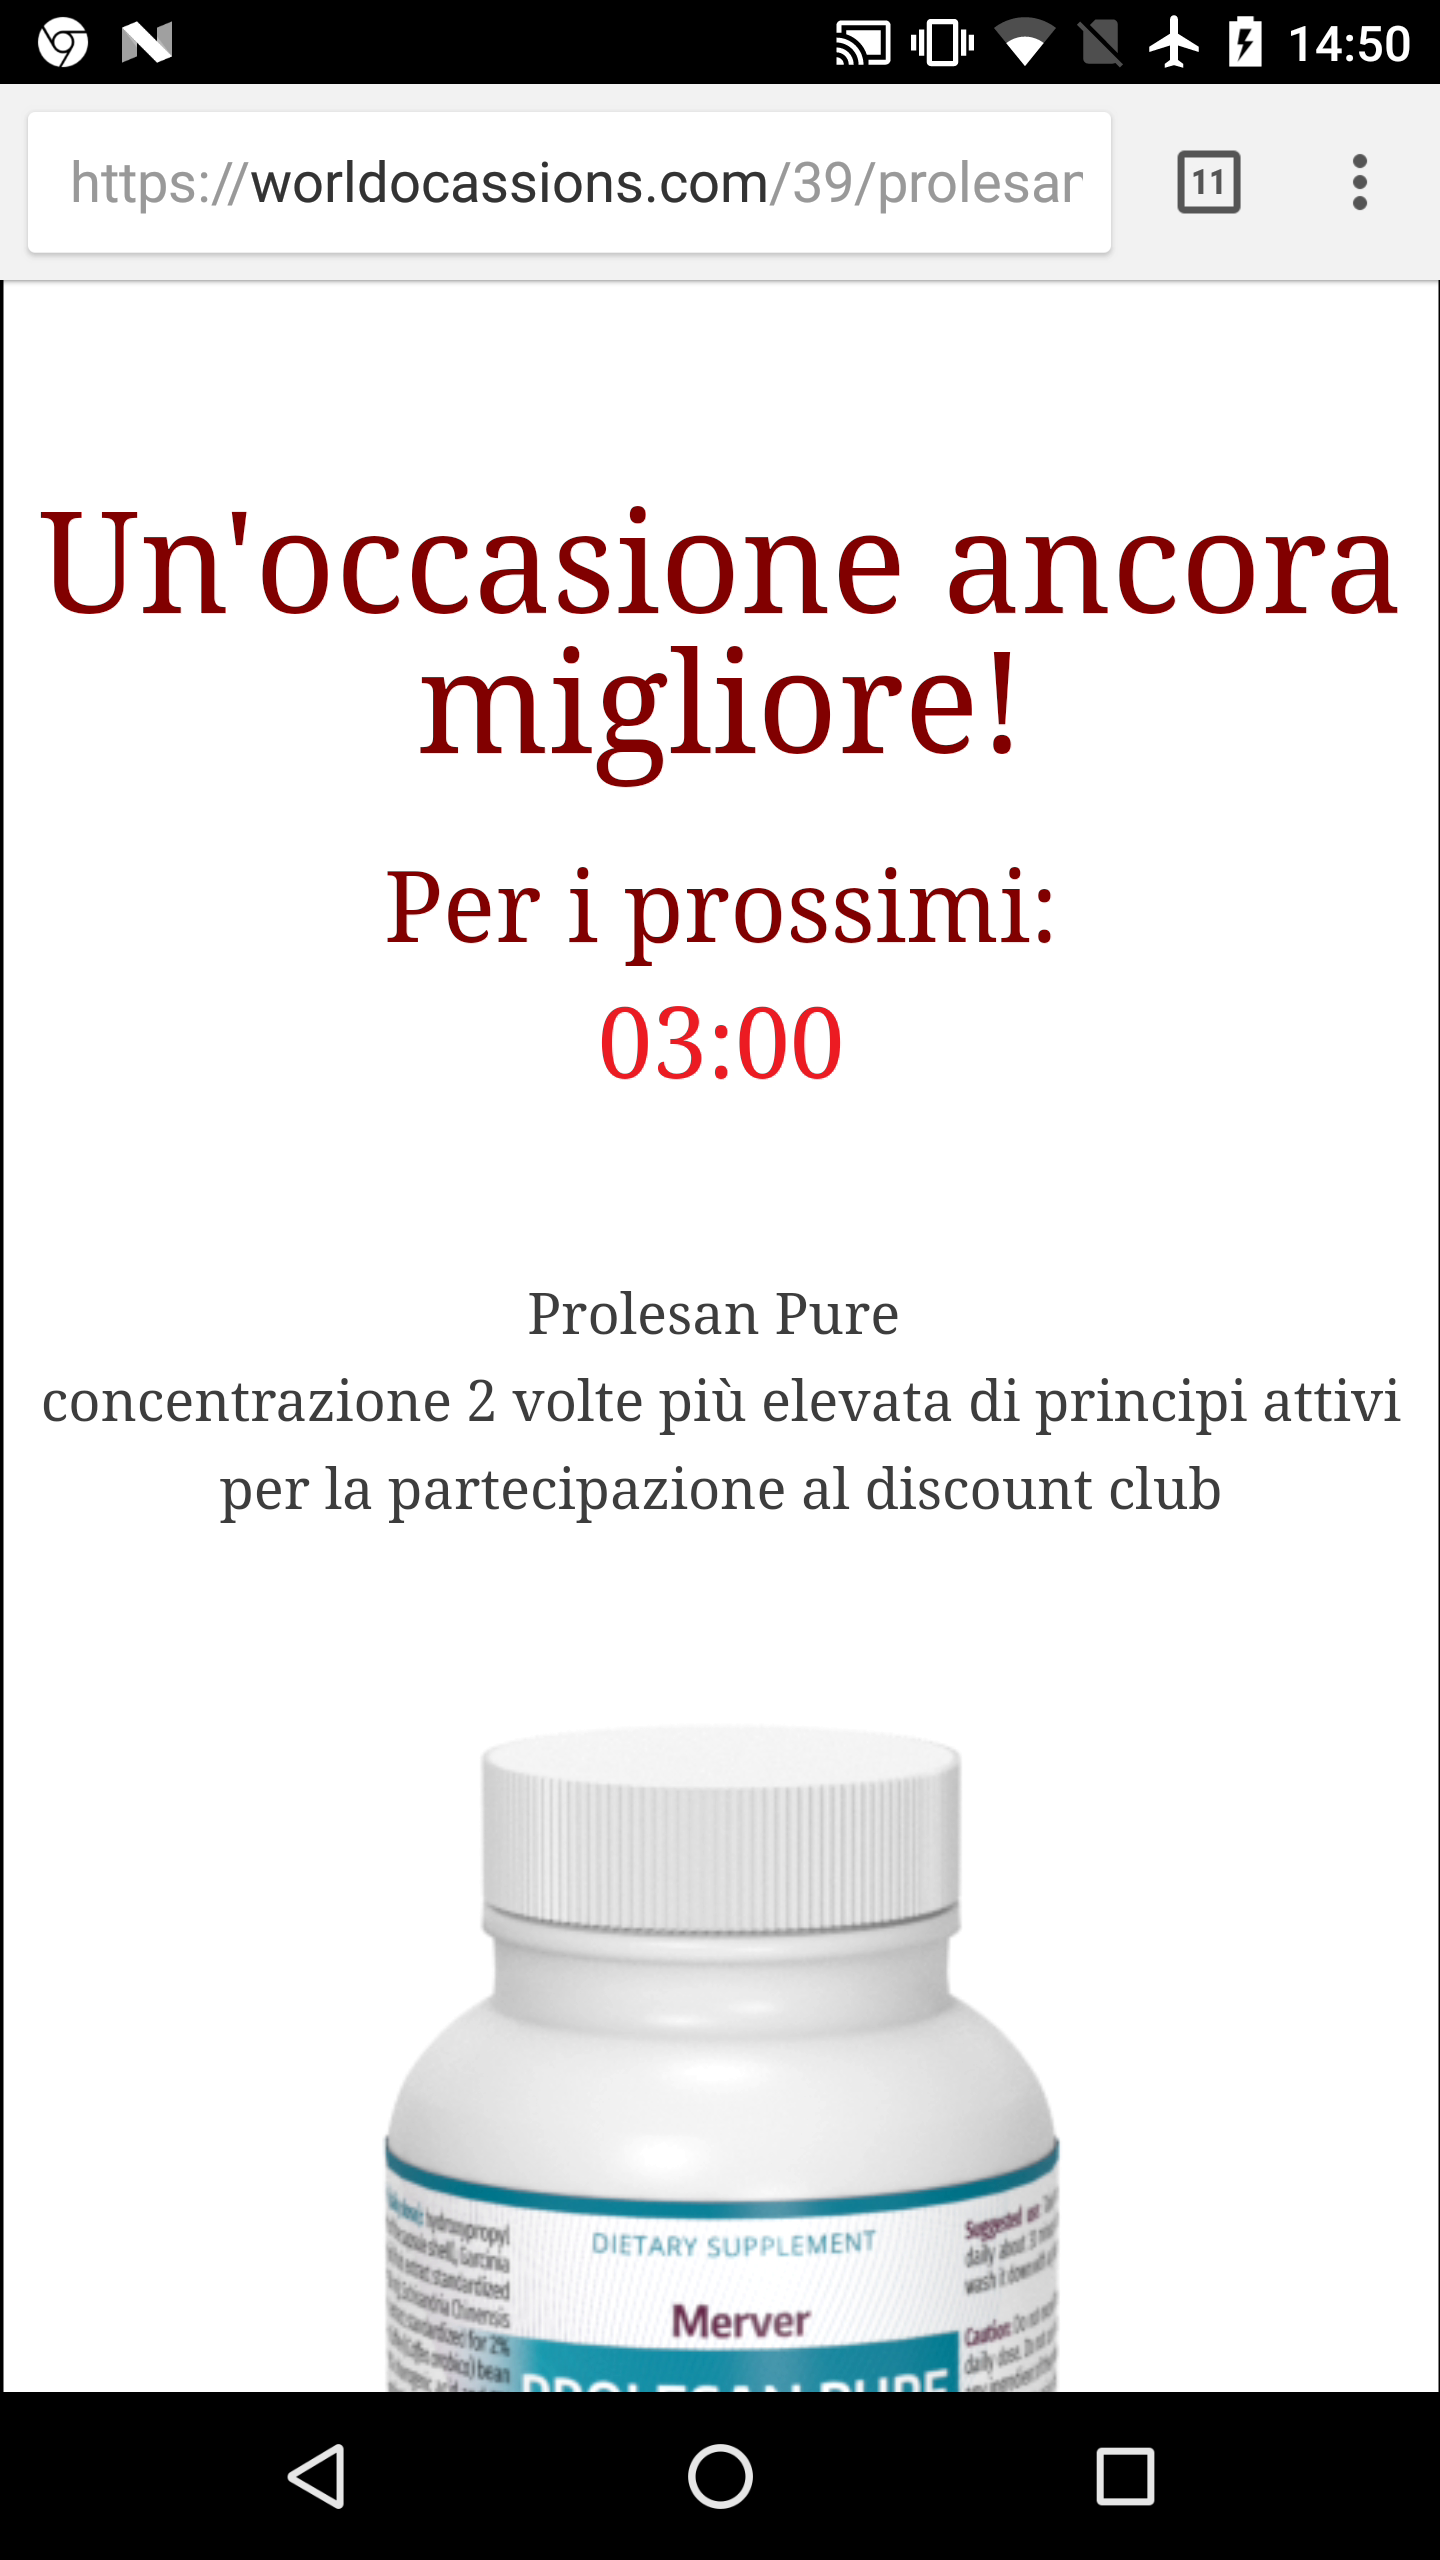
\includegraphics[scale=0.08]{figs/mobile_3}
%         \caption{Redirected Page}
%     \end{center}
%     \end{subfigure}
%     \begin{subfigure}{.24\textwidth} 
%     \begin{center}
%         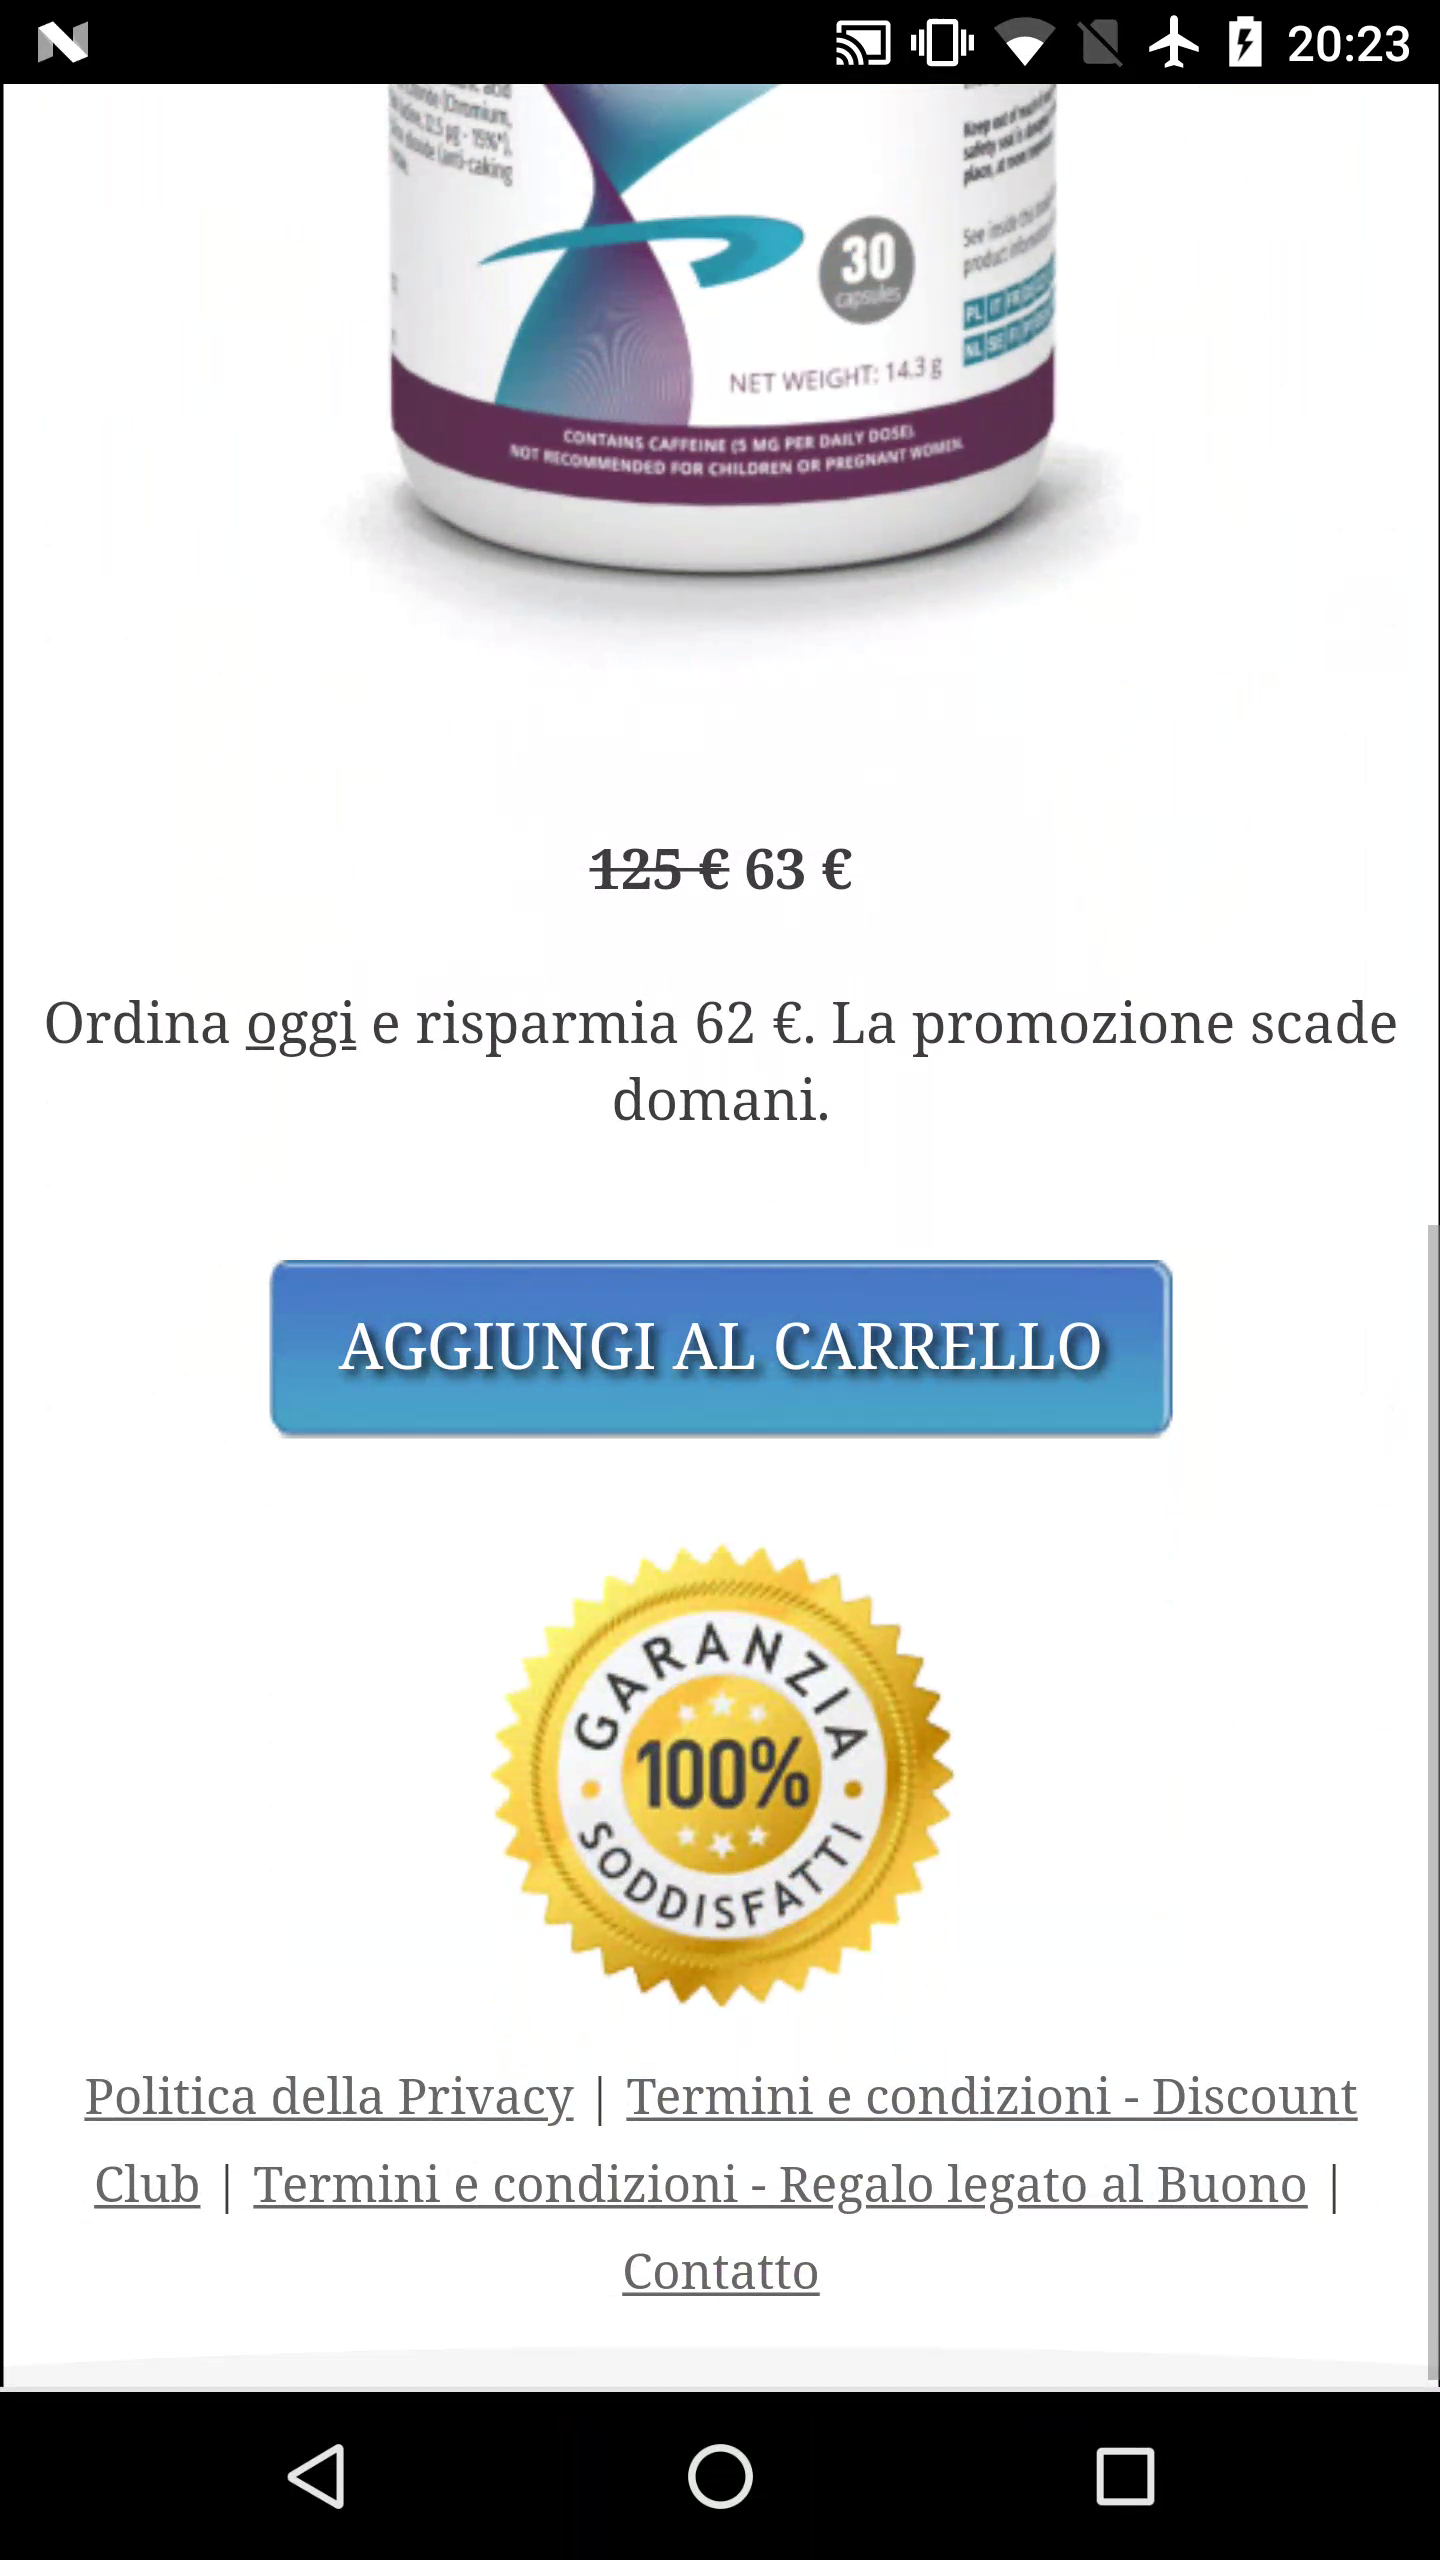
\includegraphics[scale=0.08]{figs/mobile_4}
%         \caption{Redirected Page - Cont.}
%     \end{center}
%     \end{subfigure}
%     \begin{subfigure}{.24\textwidth} 
%     \begin{center}
%         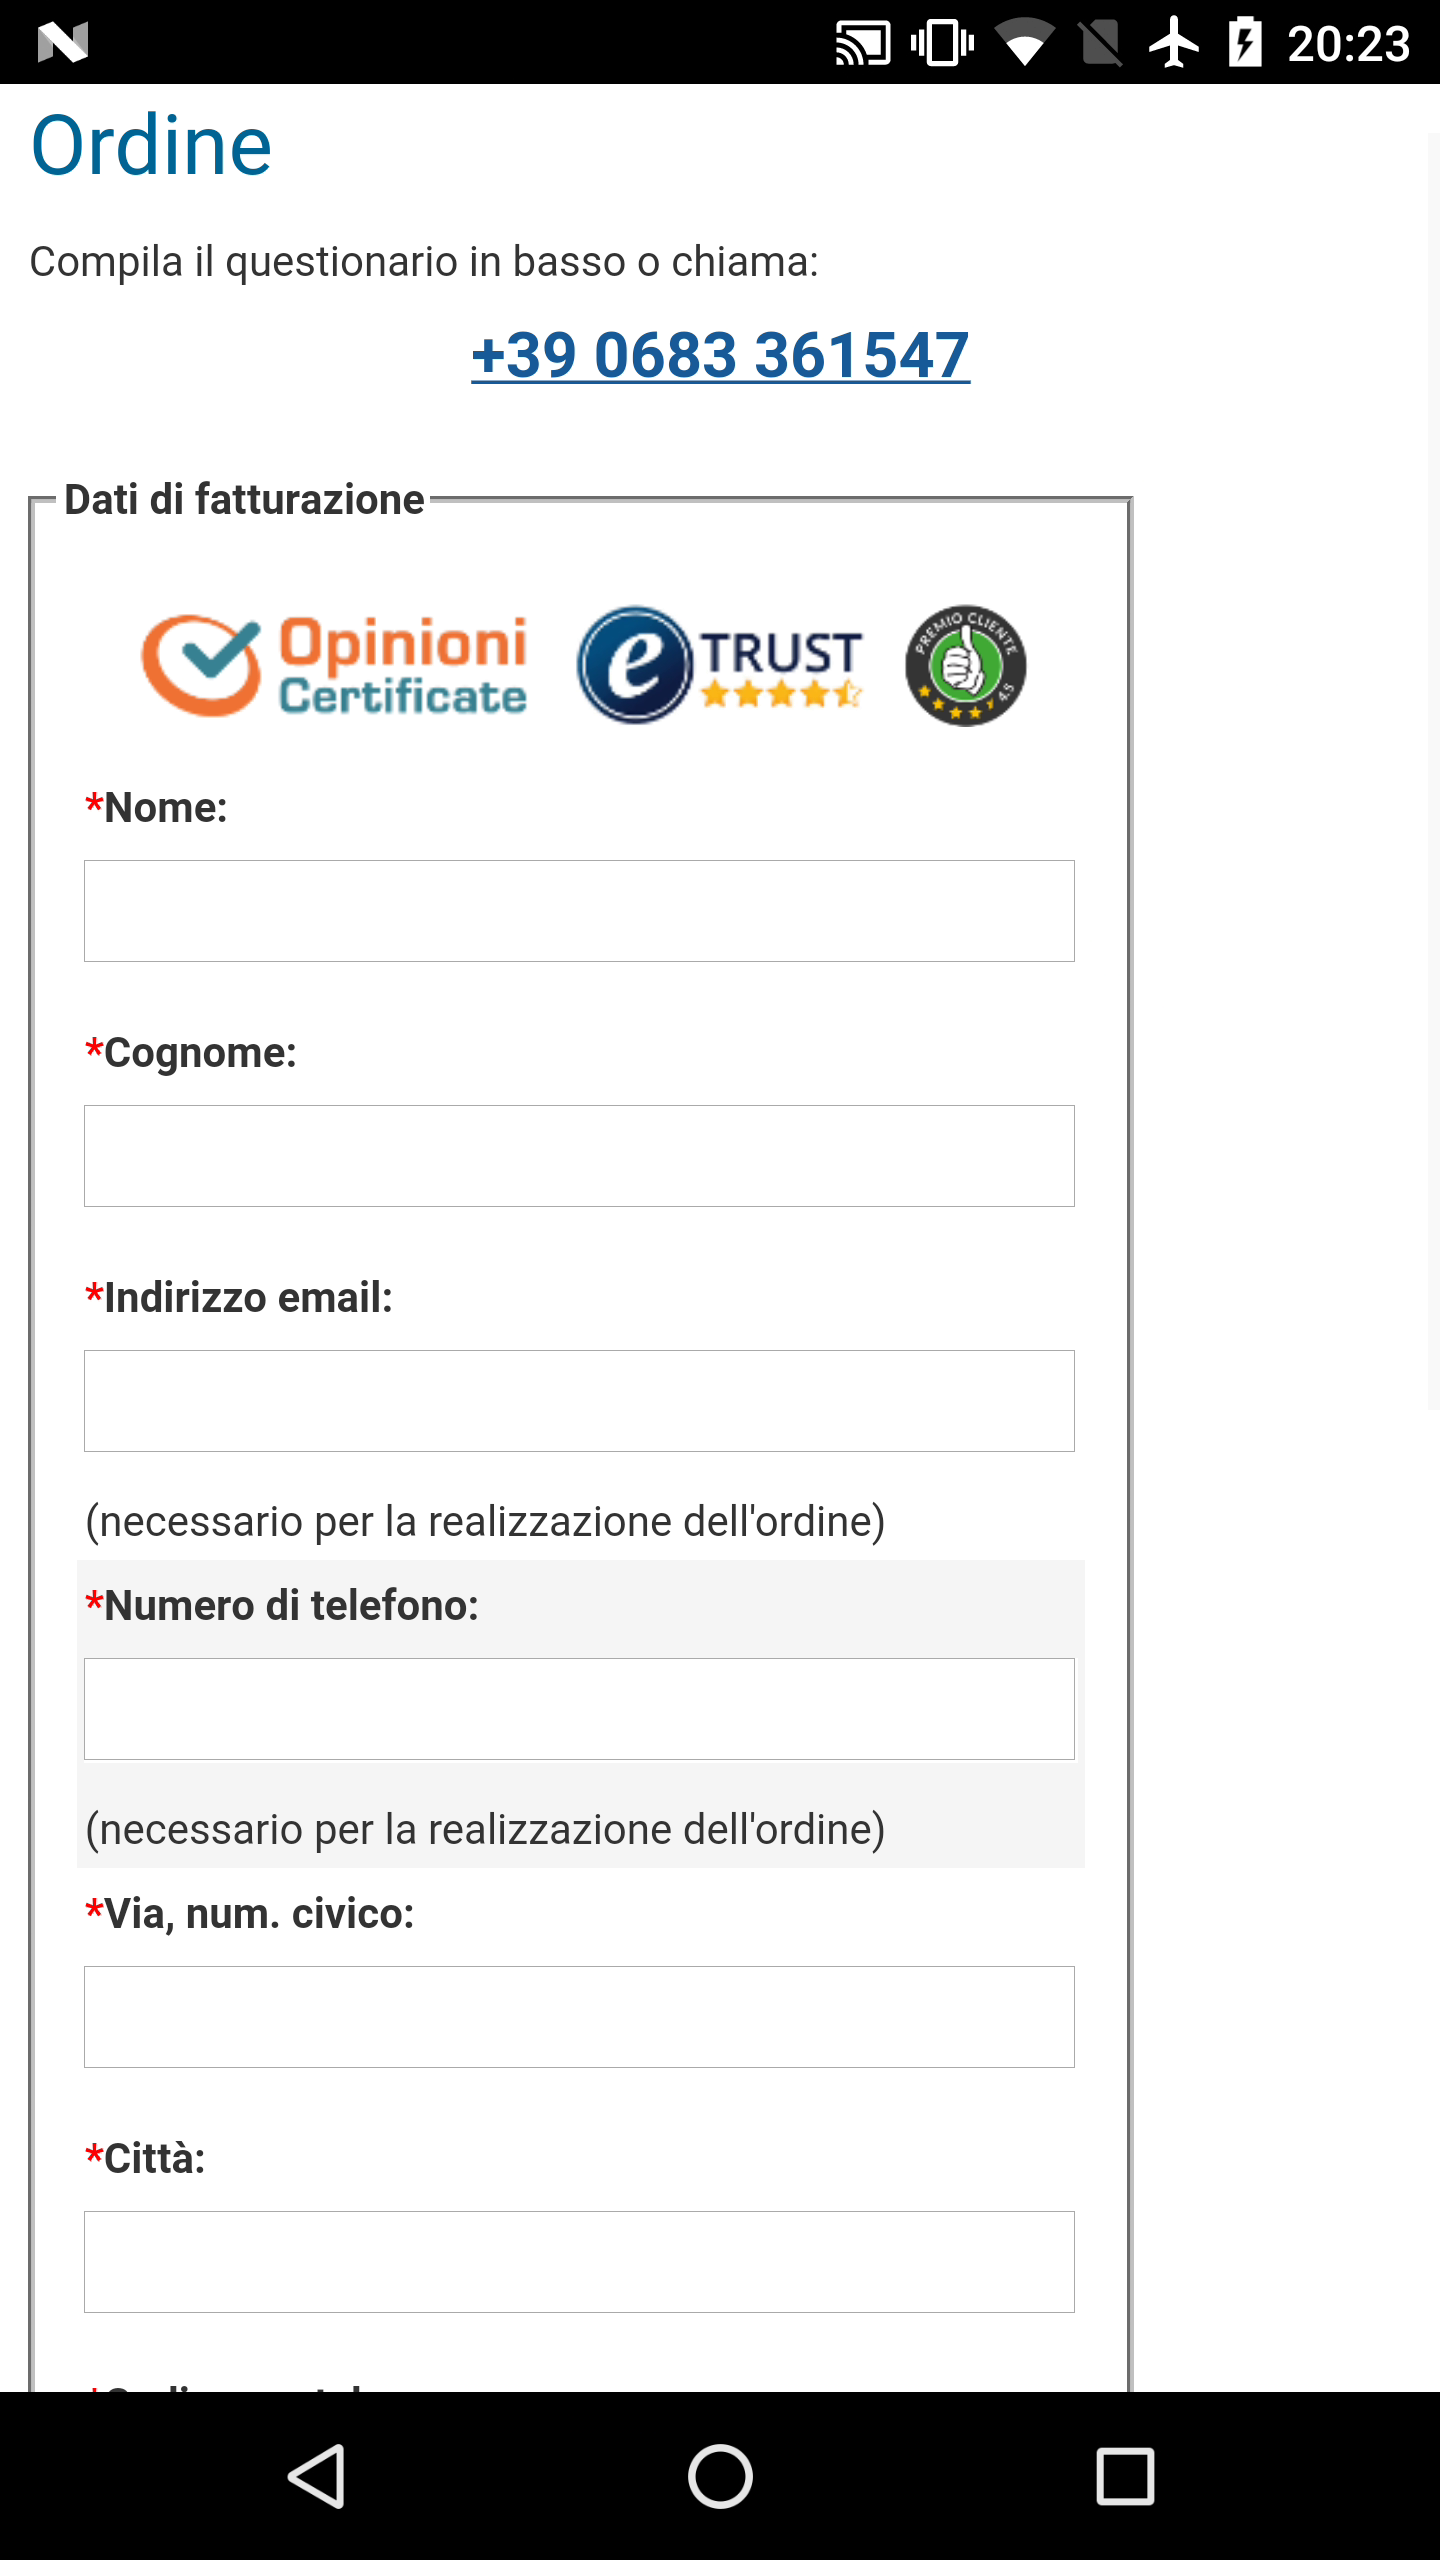
\includegraphics[scale=0.08]{figs/mobile_5}
%         \caption{Form of Sensitive Information}
%     \end{center}
%     \end{subfigure}
%     \caption{Title phishing}
%     \label{fig:mobile}
% \end{center}
% \end{figure}

% \begin{figure*}[h]
% \begin{center}
%     \begin{subfigure}{.2\textwidth}
%     \begin{center}
%         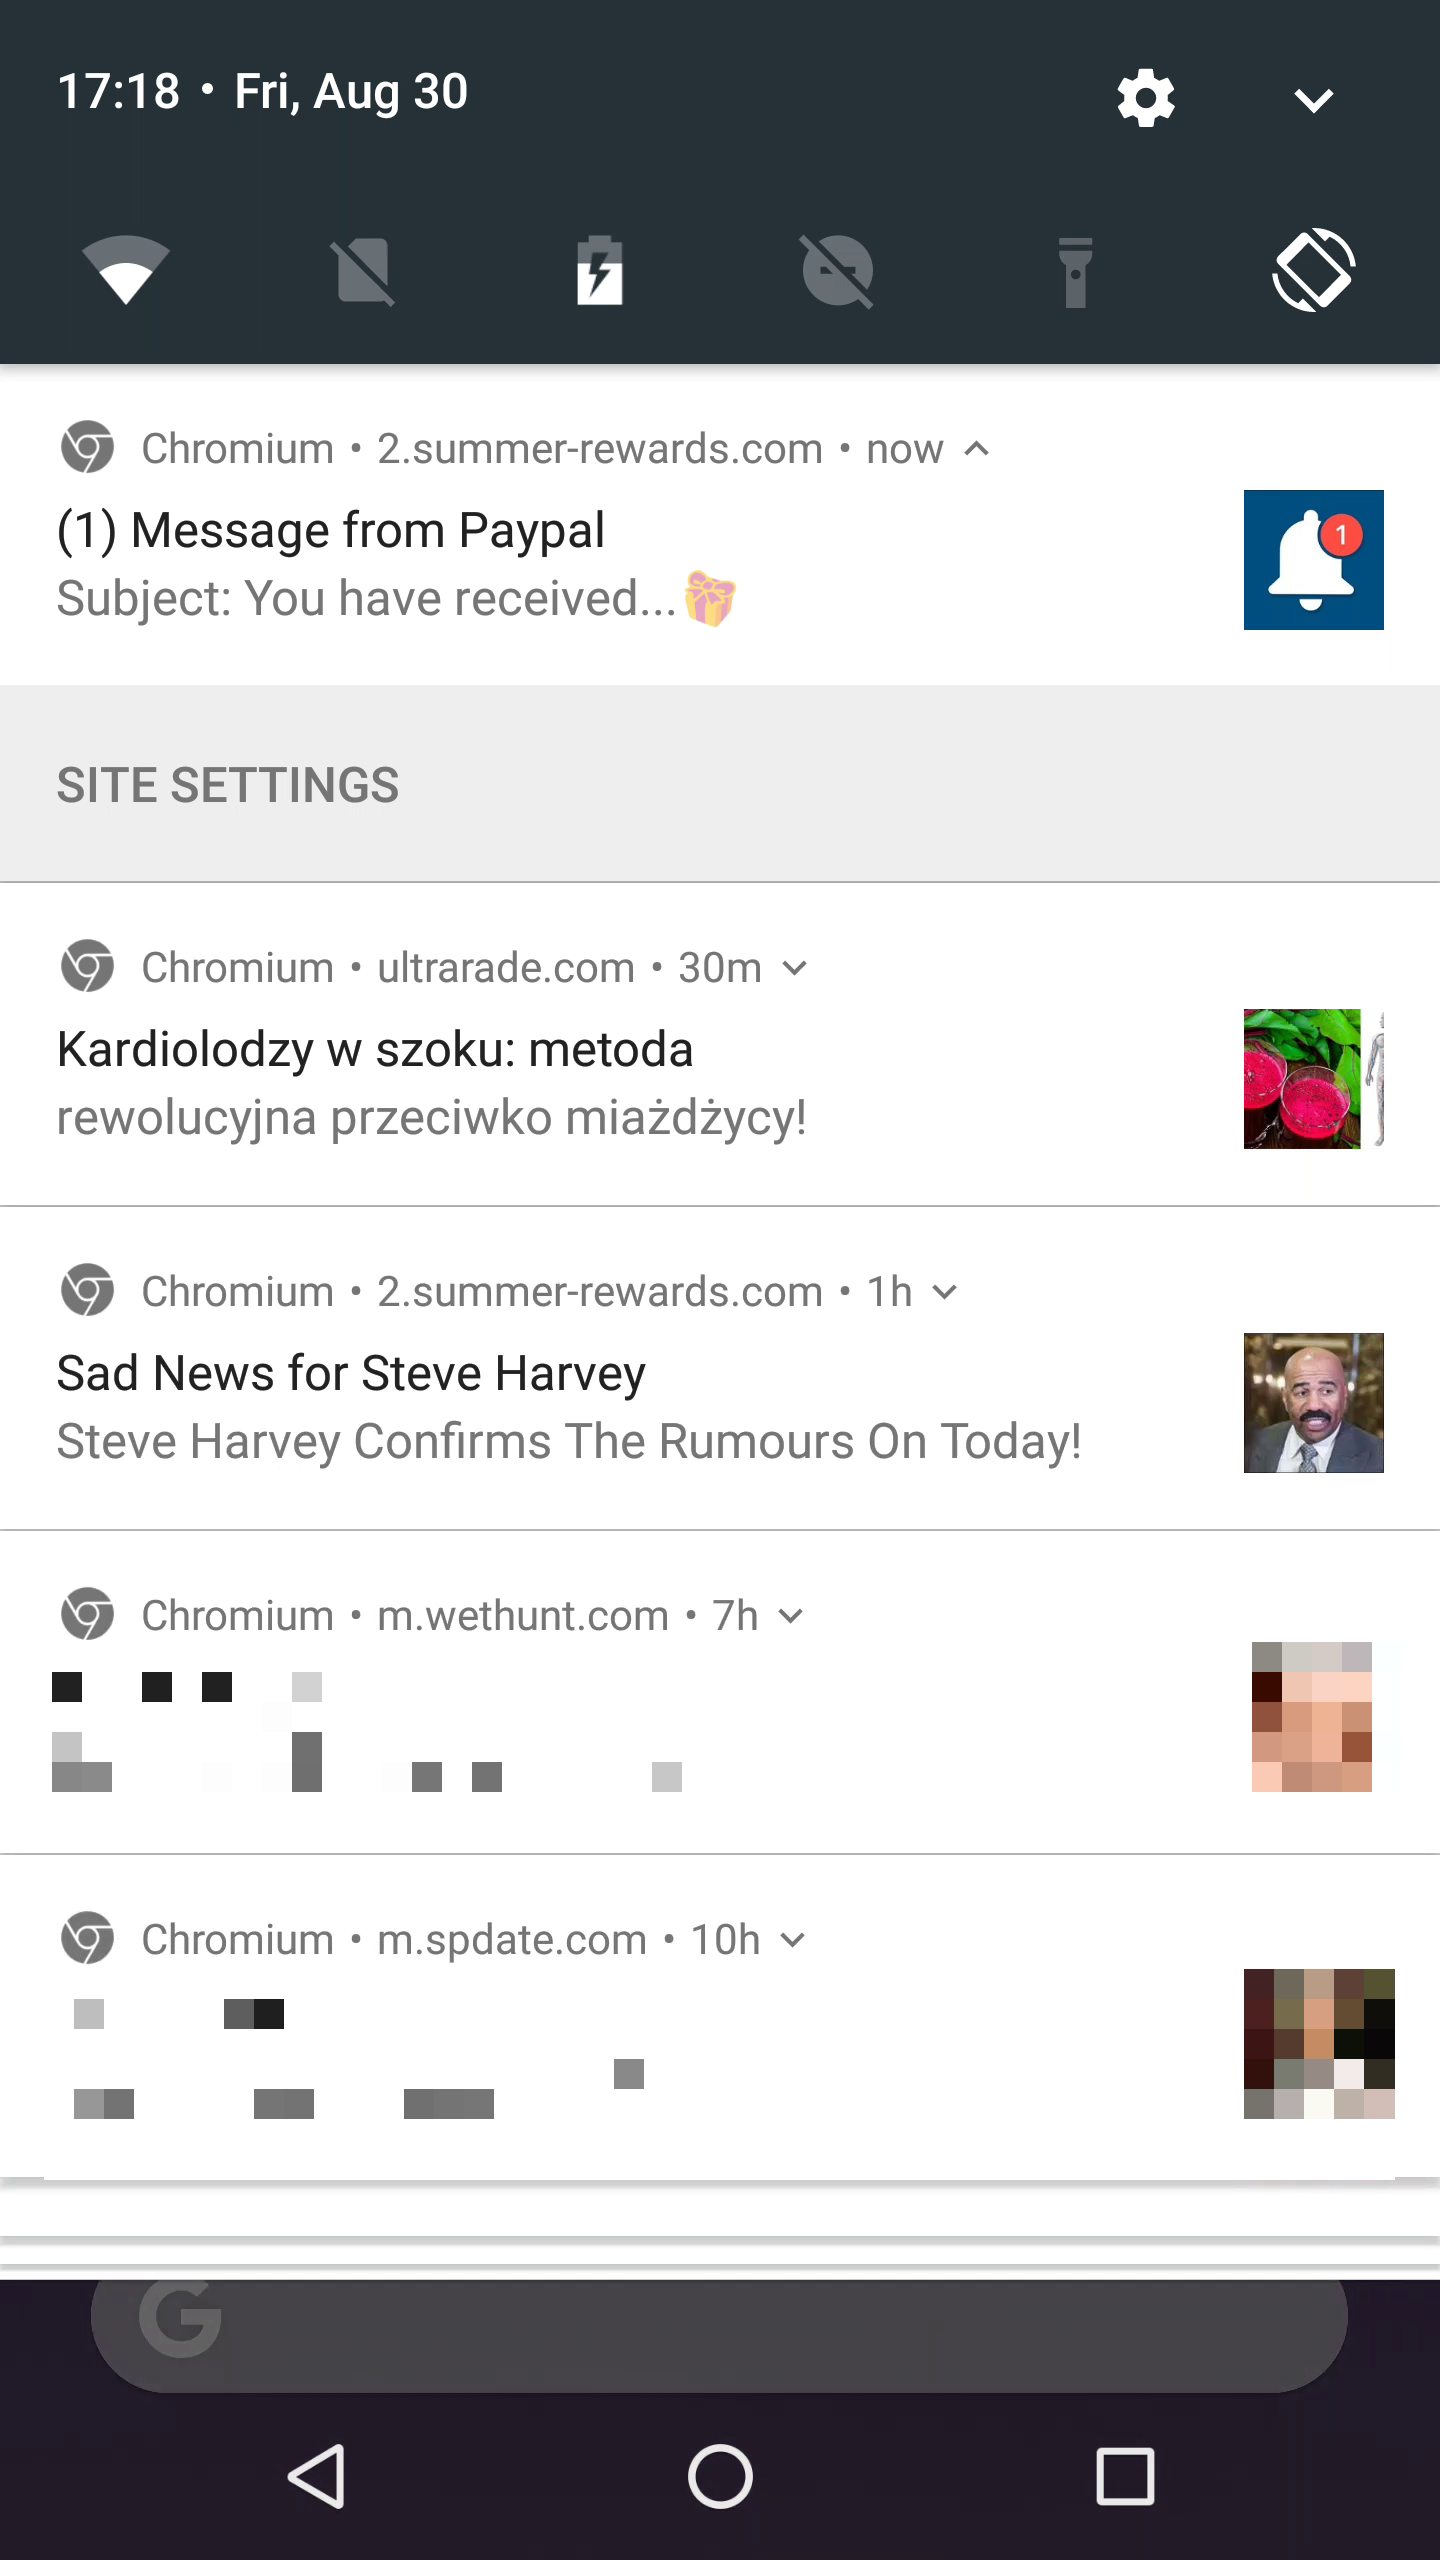
\includegraphics[width=\linewidth]{figs/mobile_disguised_1}
%         \caption{}
%     \end{center}
%     \end{subfigure}
%     \begin{subfigure}{.2\textwidth} 
%     \begin{center}
%         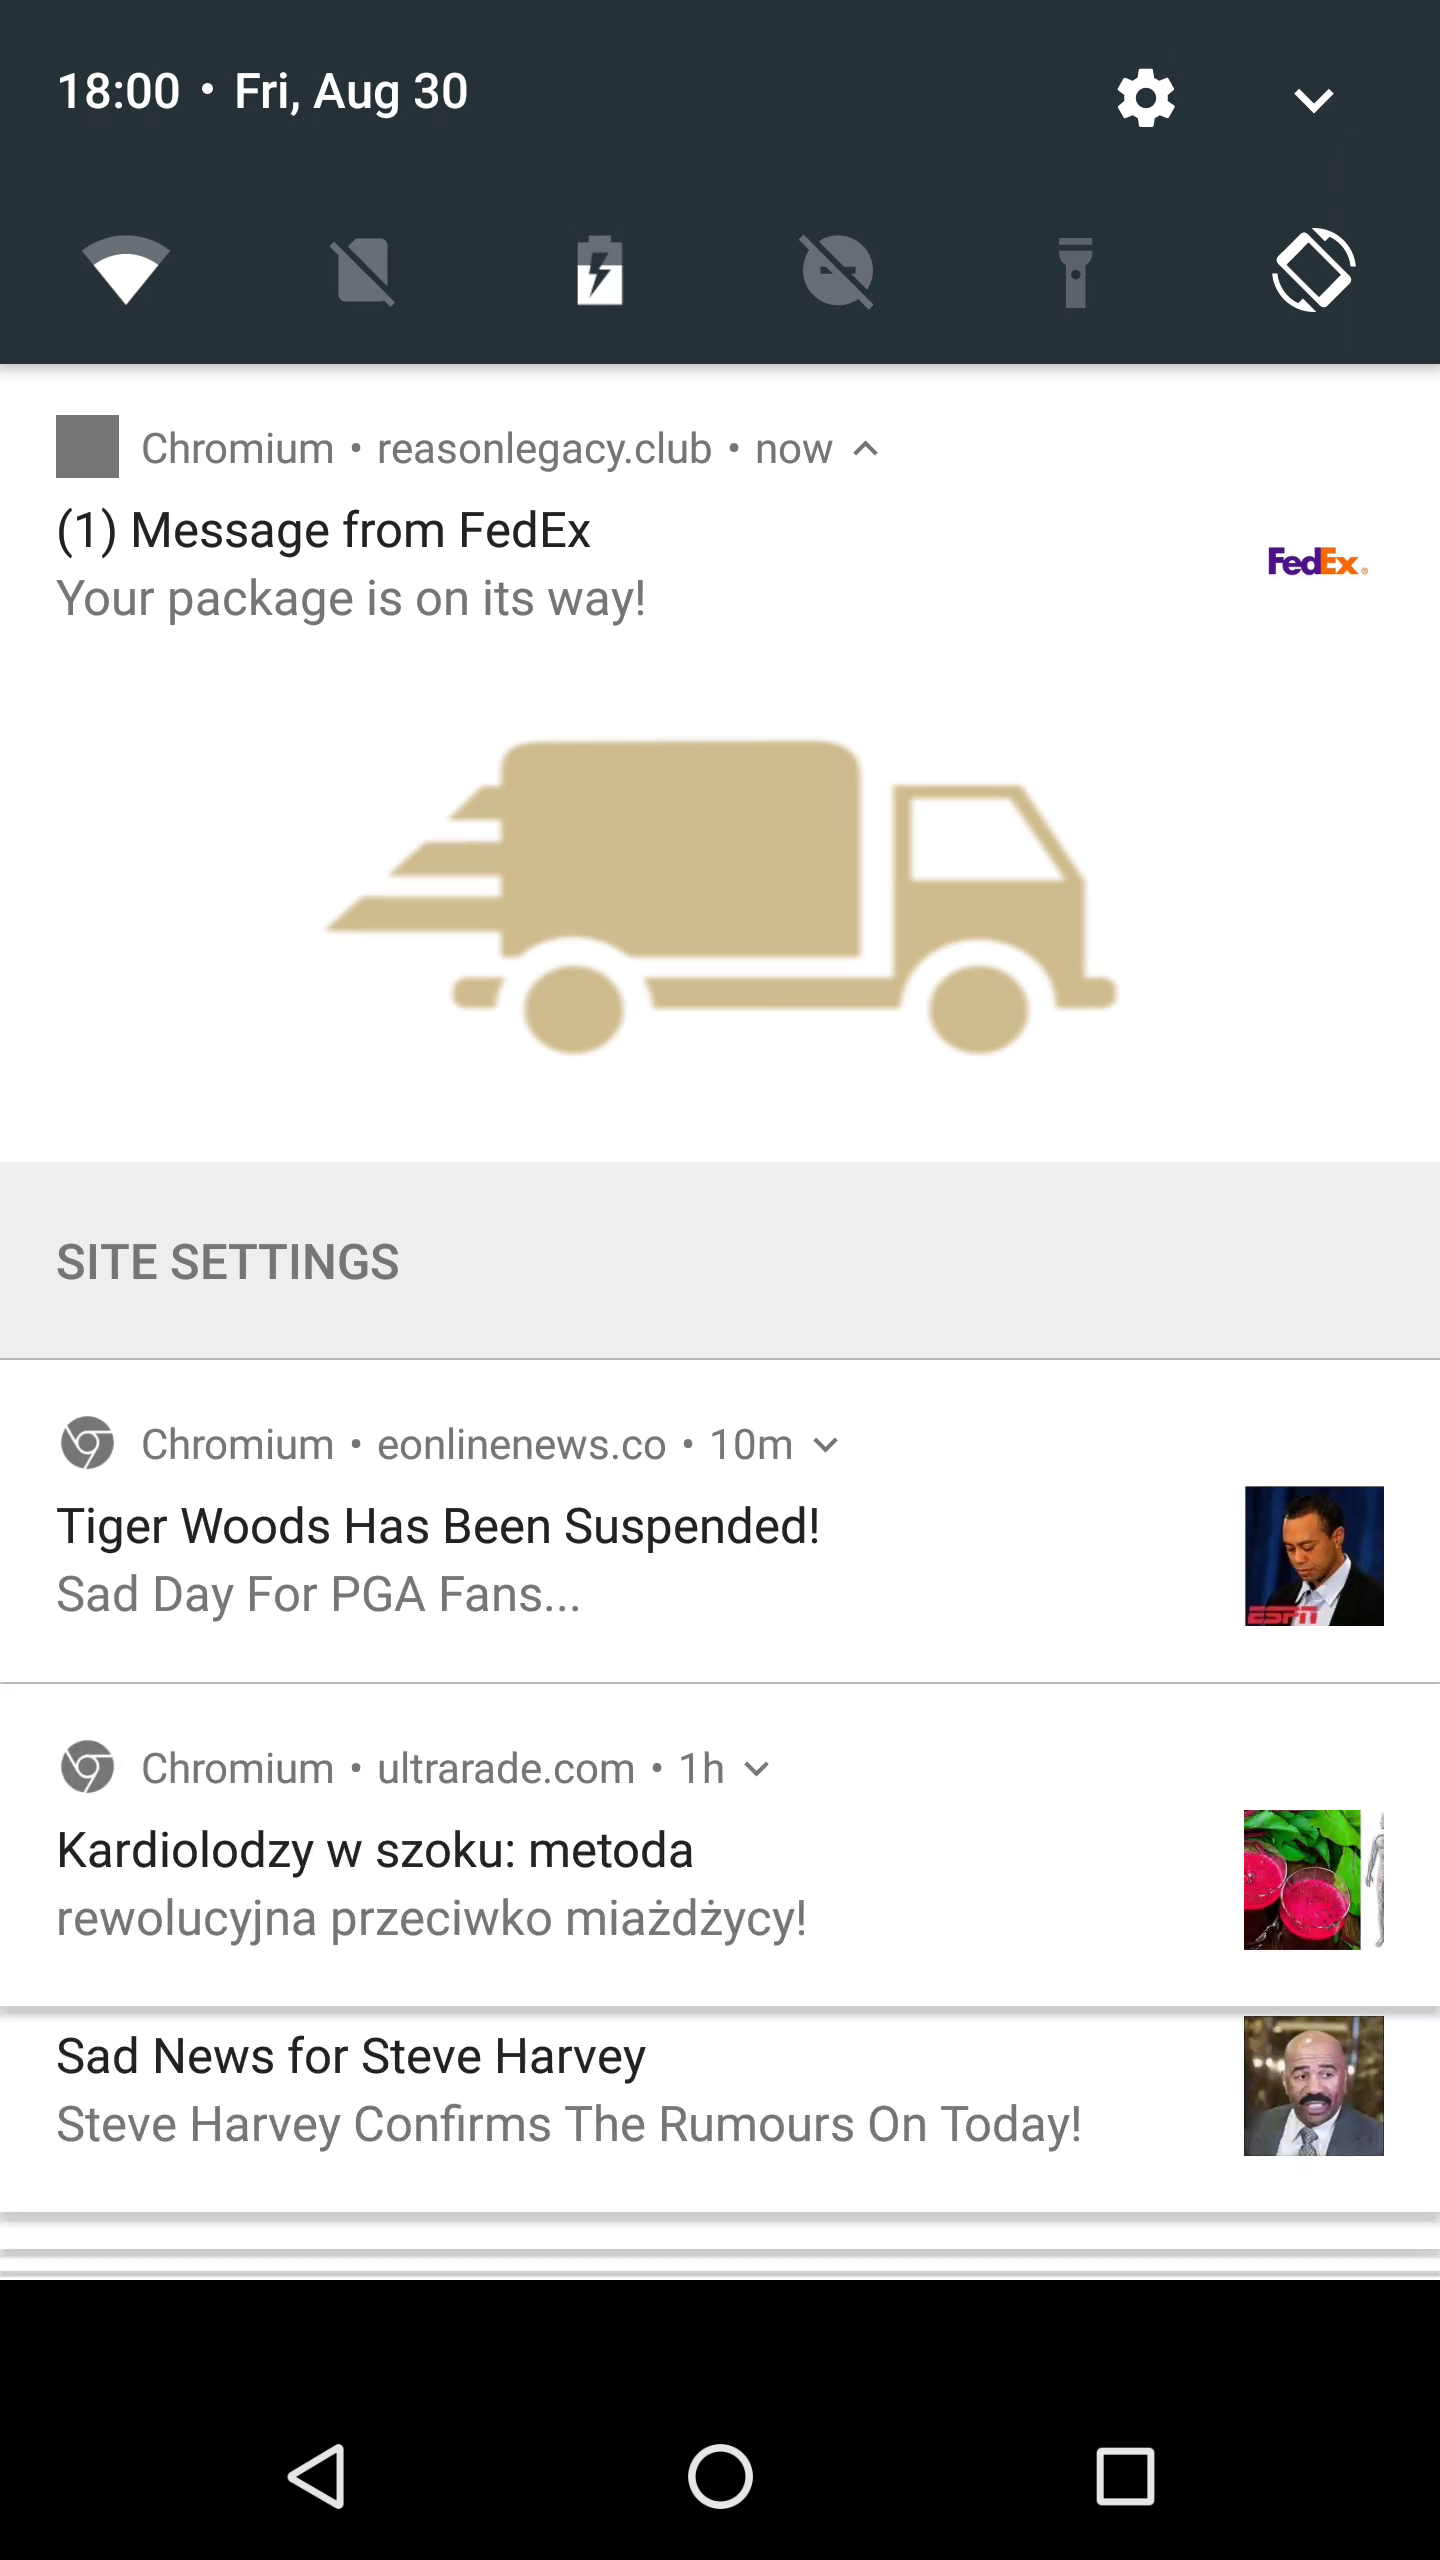
\includegraphics[width=\linewidth]{figs/mobile_disguised_2}
%         \caption{}
%     \end{center}
%     \end{subfigure}
%     \begin{subfigure}{.2\textwidth} 
%     \begin{center}
%         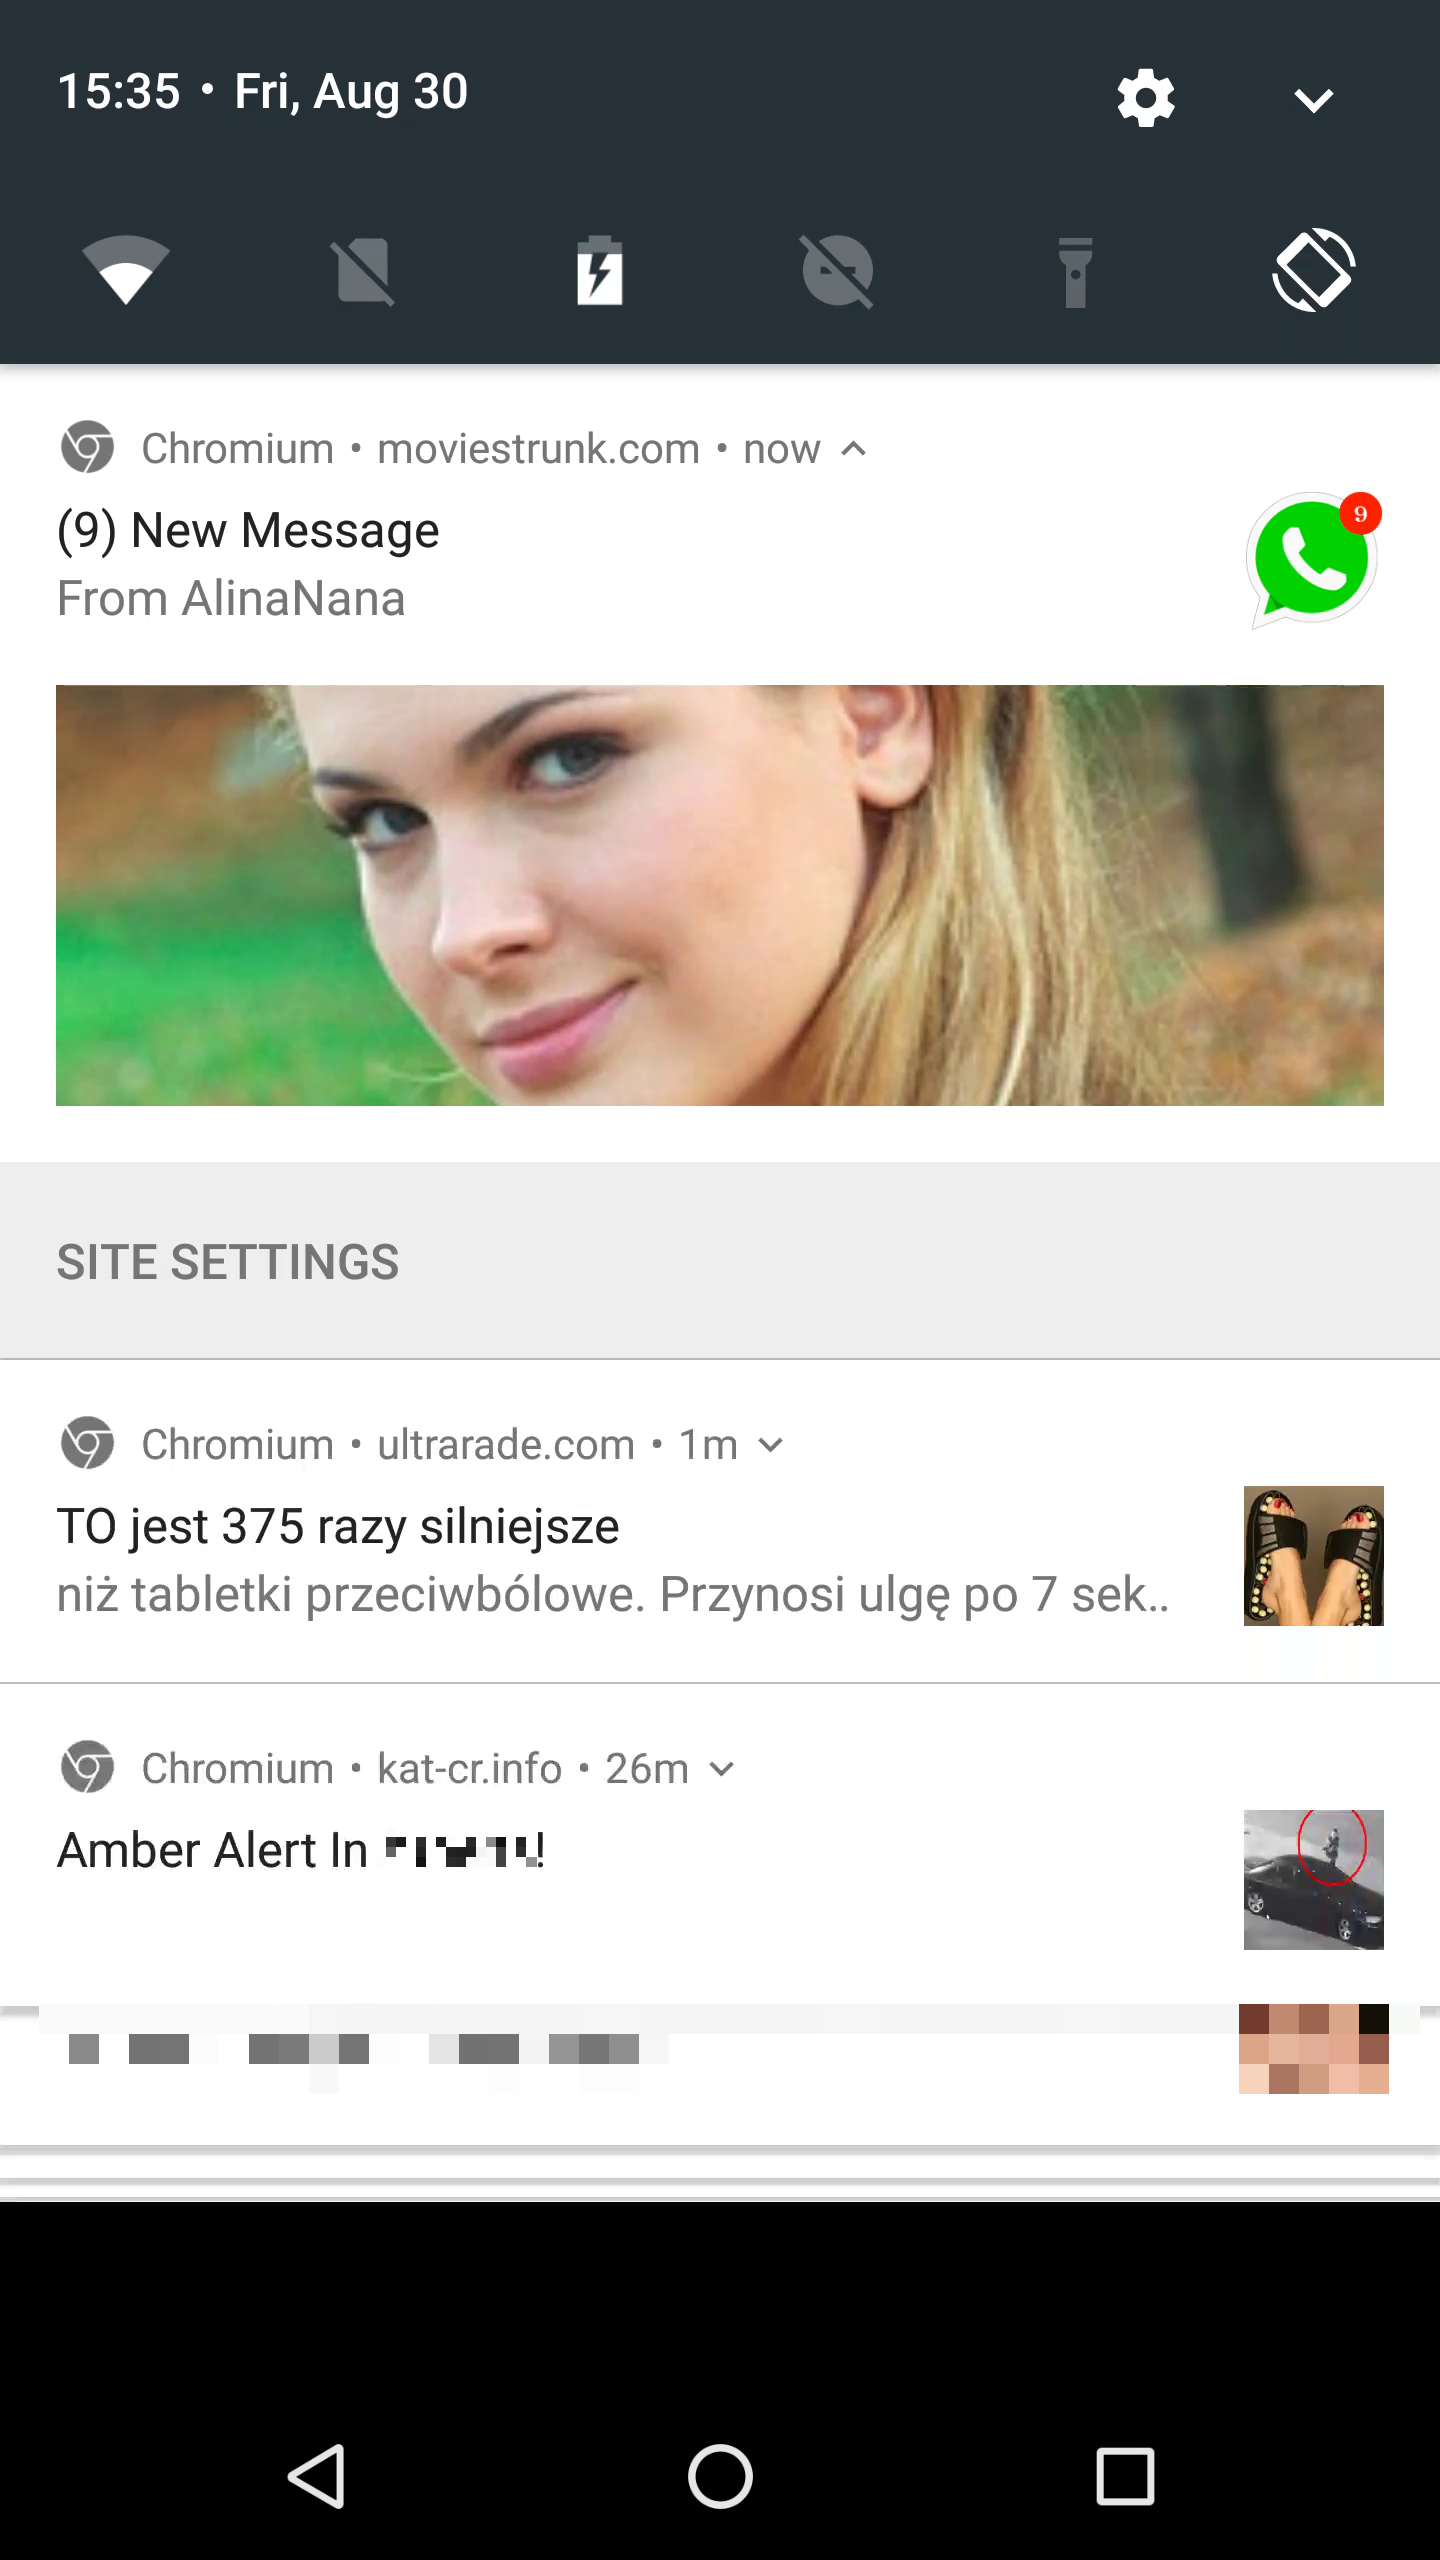
\includegraphics[width=\linewidth]{figs/mobile_disguised_3}
%         \caption{}
%         \label{fig:location}
%     \end{center}
%     \end{subfigure}
%     \caption{Title phishing: (a)Ad disguised as SMS or E-mail notification (b)Ad disguised as FedEx's application's notification (c)Ad disguised as WhatsApp's notification}
%     \label{fig:mobile_disguised_notification}
% \end{center}
% \end{figure*}

% \begin{figure}[h]
% \begin{center}
%     \begin{subfigure}{.2\textwidth}
%     \begin{center}
%         \includegraphics[width=\linewidth]{figs/mobile_phishing_2}
%         \caption{}
%         \label{mobile_phishing_2}
%     \end{center}
%     \end{subfigure}
%     \begin{subfigure}{.2\textwidth} 
%     \begin{center}
%         \includegraphics[width=\linewidth]{figs/mobile_phishing_3}
%         \caption{}
%         \label{mobile_phishing_3}
%     \end{center}
%     \end{subfigure}
%     \caption{Content phishing}
%     \label{fig:test}
% \end{center}
% \end{figure}